% Notes and solutions


% -------------------------------------------------
% Package imports
% -------------------------------------------------
\documentclass[12pt, a4paper]{article}
\usepackage[utf8]{inputenc}% Input encoding
\usepackage[english]{babel}% Set language to english
\usepackage{graphicx}% For importing graphics
\usepackage{amsthm, amsfonts, amssymb, bm}% All the AMS packages
\usepackage{mathtools}% Fixes a few AMS bugs
\usepackage[expansion=false]{microtype}% Fixes to make typography better
\usepackage{hyperref}% For \href{URL}{text}
\usepackage{fancyhdr}% For fancy headers
\usepackage[sharp]{easylist}% Easy nested lists
\usepackage{parskip}% Web-like paragraphs
\usepackage{multicol}% For multiple columns
\usepackage{tikz-cd}% For diagrams
\usepackage{microtype}
\usepackage{listings}% To include source-code
\usepackage[margin = 2.5cm, includehead]{geometry}% May be used to set margins
\usepackage{nicefrac}% Enables \nicefrac{nom}{denom}
%\usepackage[sc]{mathpazo}% A nice font, alternative to CM
\usepackage{booktabs}
\usepackage{fancyvrb} % fancy verbatim

% -------------------------------------------------
% Package setup
% -------------------------------------------------

\newcommand{\Title}{Solutions to\\``Pattern Recognition and Machine Learning''\\by Bishop}
%\newcommand{\Subtitle}{A summary of main ideas and concepts}
\newcommand{\Author}{\texttt{tommyod} @ github}
\newcommand{\listSpace}{-0.5em}% Global list space

\title{\Title}
\author{\Author}

% Shortcuts for sets and other stuff in mathematics
\newcommand{\Q}{\mathbb{Q}}
\newcommand{\R}{\mathbb{R}}
\newcommand{\C}{\mathbb{C}}
\newcommand{\D}{\mathcal{D}}
\newcommand{\F}{\mathcal{F}}
\newcommand{\Y}{\mathcal{Y}}
\newcommand{\Reg}{\mathcal{R}}
\newcommand{\Class}{\mathcal{C}}
\newcommand{\Z}{\mathbb{Z}}
\renewcommand{\sf}[1]{\mathsf{#1}}
\newcommand{\vect}[1]{\bm{#1}}
\newcommand{\norm}[1]{\left\lVert#1\right\rVert}
\newcommand{\abs}[1]{\left\lvert#1\right\rvert}

% Shortcuts for probability distributions
\DeclareMathOperator{\N}{\mathcal{N}}
\DeclareMathOperator{\Bern}{\operatorname{Bern}}
\DeclareMathOperator{\Gam}{\operatorname{Gam}}
\DeclareMathOperator{\Beta}{\operatorname{Beta}}
\DeclareMathOperator{\Bin}{\operatorname{Bin}}
\DeclareMathOperator{\St}{\operatorname{St}}
\DeclareMathOperator{\U}{\operatorname{U}}
\DeclareMathOperator{\KL}{\operatorname{KL}}

% Shortcuts for statistical operators
\DeclareMathOperator{\E}{\mathbb{E}}
\DeclareMathOperator{\var}{\operatorname{var}}
\DeclareMathOperator{\cov}{\operatorname{cov}}
\DeclareMathOperator{\SD}{\operatorname{SD}}
\renewcommand{\H}{\operatorname{H}}


% -------------------------------------------------
% Document start
% -------------------------------------------------
\begin{document}
	
\maketitle
\begin{abstract}
This document contains some notes and solutions to the book TODO.

\begin{figure}[ht!]
	\centering
	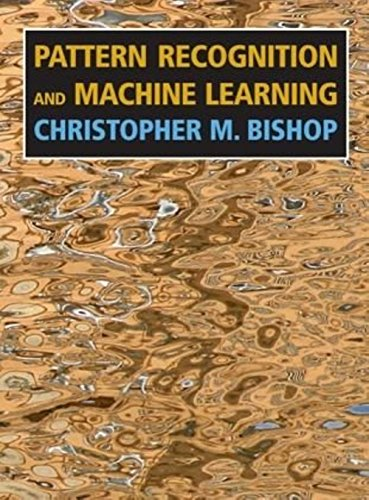
\includegraphics[width=0.25\linewidth]{figs/bishop}
	\caption{The front cover of \cite{bishop_pattern_2011}.}
	\label{fig:duda}
\end{figure}
\end{abstract}

\clearpage

{\small \tableofcontents}


\clearpage
\section{Chapter notes}

% ----------------------------------------------------------------------------
\subsection{Introduction}
\begin{easylist}[itemize]
	\ListProperties(Space=\listSpace, Space*=\listSpace, Numbers1=l, FinalMark1={)})
	# sdf
\end{easylist}

% ----------------------------------------------------------------------------
\subsection{Probability Distributions}
\begin{easylist}[itemize]
	\ListProperties(Space=\listSpace, Space*=\listSpace, Numbers1=l, FinalMark1={)})
	# sdf
\end{easylist}

% ----------------------------------------------------------------------------
\subsection{Linear Models for Regression}
\begin{easylist}[itemize]
	\ListProperties(Space=\listSpace, Space*=\listSpace, Numbers1=l, FinalMark1={)})
	# sdf
\end{easylist}

% ----------------------------------------------------------------------------
\subsection{Linear Models for Classification}
\begin{easylist}[itemize]
	\ListProperties(Space=\listSpace, Space*=\listSpace, Numbers1=l, FinalMark1={)})
	# sdf
\end{easylist}

% ----------------------------------------------------------------------------
\subsection{Neural networks}
\begin{easylist}[itemize]
	\ListProperties(Space=\listSpace, Space*=\listSpace, Numbers1=l, FinalMark1={)})
	# sdf
\end{easylist}

% ----------------------------------------------------------------------------
\subsection{Kernel methods}
\begin{easylist}[itemize]
	\ListProperties(Space=\listSpace, Space*=\listSpace, Numbers1=l, FinalMark1={)})
	# sdf
\end{easylist}

% ----------------------------------------------------------------------------
\subsection{Sparse Kernel Machines}
\begin{easylist}[itemize]
	\ListProperties(Space=\listSpace, Space*=\listSpace, Numbers1=l, FinalMark1={)})
	# sdf
\end{easylist}

% ----------------------------------------------------------------------------
\subsection{Graphical Models}
\begin{easylist}[itemize]
	\ListProperties(Space=\listSpace, Space*=\listSpace, Numbers1=l, FinalMark1={)})
	# sdf
\end{easylist}

% ----------------------------------------------------------------------------
\subsection{Mixture Models and EM}
\begin{easylist}[itemize]
	\ListProperties(Space=\listSpace, Space*=\listSpace, Numbers1=l, FinalMark1={)})
	# sdf
\end{easylist}

% ----------------------------------------------------------------------------
\subsection{Approximate Interference}
\begin{easylist}[itemize]
	\ListProperties(Space=\listSpace, Space*=\listSpace, Numbers1=l, FinalMark1={)})
	# sdf
\end{easylist}

% ----------------------------------------------------------------------------
\subsection{Sampling Methods}
\begin{easylist}[itemize]
	\ListProperties(Space=\listSpace, Space*=\listSpace, Numbers1=l, FinalMark1={)})
	# sdf
\end{easylist}

% ----------------------------------------------------------------------------
\subsection{Continuous Latent Variables}
\begin{easylist}[itemize]
	\ListProperties(Space=\listSpace, Space*=\listSpace, Numbers1=l, FinalMark1={)})
	# sdf
\end{easylist}

% ----------------------------------------------------------------------------
\subsection{Sequential Data}
\begin{easylist}[itemize]
	\ListProperties(Space=\listSpace, Space*=\listSpace, Numbers1=l, FinalMark1={)})
	# sdf
\end{easylist}

% ----------------------------------------------------------------------------
\subsection{Combining Models}
\begin{easylist}[itemize]
	\ListProperties(Space=\listSpace, Space*=\listSpace, Numbers1=l, FinalMark1={)})
	# sdf
\end{easylist}

% ----------------------------------------------------------------------------





\clearpage

\section{Chapter summaries}

\subsubsection*{Notation}
Scalar data is given by $\mathsf{x} = \left(x_1, \dots, x_N\right)^T$, where $N$ is the number of samples. 
Vector data is given by $\vect{X}$, which has dimensions $N \times M$, where $N$ is the number of data points (rows) and $M$ is the dimensionality of the feature space (columns).

\subsubsection*{Mathematics}
Some useful mathematics is summarized here, also see the book appendix.
\begin{easylist}[itemize]
	\ListProperties(Space=\listSpace, Space*=\listSpace)
	# The \emph{gamma function} $\Gamma(x)$ satisfies $\Gamma(x) = (x-1) \Gamma(x-1)$, and is given by
	\begin{equation*}
	\Gamma(x) = \int_{0}^{\infty} u^{x-1} e^{-u}  \, du.
	\end{equation*}
	It's a ``continuous factorial,'' which is proved by integration by parts and induction.
	
	# The \emph{Jensen inequality} states that, for convex functions
	\begin{equation*}
	f\left( \sum_j \lambda_j x_j\right) \leq \sum_j \lambda_j f(x_j),
	\end{equation*}
	where $\sum_j \lambda_j = 1$ and $\lambda_j \geq 0$ for every $j$.
\end{easylist}

% ----------------------------------------------------------------------------
\subsection{Introduction}


\subsubsection*{Probability}
The joint probability is given by $p(x, y)$, which is short notation for $p(X = x_i \cap Y = y_j)$.
\begin{easylist}[itemize]
	\ListProperties(Space=\listSpace, Space*=\listSpace)
	# The sum rule is 
	\begin{equation*}
	p(x) = \sum_y p(x, y) = \int p(x, y) \, dy.
	\end{equation*}
	## Applying the sum rule as above is called ``marginalizing out $y$.''
	# The product rule is 
	\begin{equation*}
	p(x, y) = p(x | y) p(y).
	\end{equation*}
	## Computing $p(x | y)$ is called ``conditioning on $y$.''
	# Let $\vect{w}$ be parameters and $\D$ be data.
	Bayes theorem is given by
	\begin{equation*}
	p(\vect{w} | \D) = \frac{p(\D | \vect{w}) p(\vect{w})}{p(\D)} \quad \Leftrightarrow \quad
	\text{posterior} = \frac{\text{likelihood} \times \text{prior}}{\text{evidence}}.
	\end{equation*}
	
	## Frequentist: data $\D$ generated from a fixed $\vect{w}$.
	## Bayesian: data $\D$ fixed, find best $\vect{w}$ given this data.
	# Frequentists generally quantify the properties of data driven
	quantities in light of the fixed model parameters,
	while Bayesians generally quantify the properties of unknown
	model parameters in light of observed data.
	See \cite{vanderplas_frequentism_2014}.
\end{easylist}

\subsubsection*{Expectation and covariance}
Let $x$ be distributed with density $p(x)$, then
\begin{easylist}[itemize]
	\ListProperties(Space=\listSpace, Space*=\listSpace)
	# The expectation of a function $f(x)$ defined over $x$ with probability density $p(x)$ is
	\begin{equation*}
	\E[f] = \sum_j f(x_j) p (x_j) = \int f(x) p(x) \, dx
	\end{equation*}
	# The variance of $f(x)$ is
	\begin{equation*}
	\var[f] = \E \left[ (f - \E[f])^2\right] = \E[f^2] - \E[f]^2
	\end{equation*}
	# The covariance of $x$ and $y$ given by
	\begin{equation*}
	\cov[x, y] = \E_{x,y} \left[ (x - \E[x]) (y - \E[y])\right]
	\end{equation*}
	# The covariance matrix $\mathbf{\Sigma}$ has entries $\sigma_{ij}$ corresponding to the covariance of variables $i$ and $j$.
	Thus $\vect{\Sigma} = \vect{I}$ means no covariance.
	(Note that real data may have no covariance and still be dependent, i.e. have predictive power, $x_j = f(x_k)$ where $f$ is non-linear.
	See ``Anscombe's quartet'' on Wikipedia.)
\end{easylist}

\subsubsection*{Polynomial fitting}
Let $y(x, \vect{w}) = \sum_{j = 1}^{M} w_j x^j$ be a polynomial.
We wish to fit this polynomial to values $\sf{x} = \left(x_1, \dots, x_N\right)$ and $\sf{t} = \left(t_1, \dots, t_N\right)$
i.e. a degree $M$ polynomial fitting $N$ data points.

\begin{easylist}[itemize]
	\ListProperties(Space=\listSpace, Space*=\listSpace)
	# The maximum likelihood solution is to minimize
	\begin{equation*}
	E(\vect{w}, \mathsf{x}) \propto \sum_{n = 1}^{N} \left[ y (x_n, \vect{w}) - t_n\right]^2.
	\end{equation*}
	# Regularization adds a weight-dependent error so that $\widetilde{E}(\vect{w}, \mathsf{x}) = E(\vect{w}, \mathsf{x}) + E(\vect{w})$.
	For instance, Ridge minimizes the $2$-norm:
	\begin{equation*}
	\widetilde{E}(\vect{w}, \mathsf{x}) \propto \sum_{n = 1}^{N} \left[ y (x_n, \vect{w}) - t_n\right]^2 + \lambda \norm{\vect{w}}_2^2
	\end{equation*}
	While LASSO (Least Absolute Shrinkage and Selection Operator) minimizes and error with the $1$-norm.
	Both are examples of \emph{Tikhonov regularization}.
\end{easylist}

\subsubsection*{Gaussians}
The multivariate Gaussian is given by
\begin{equation*}
\N\left(x | \vect{\mu}, \vect{\Sigma}\right) = 
\frac{1}{(2\pi)^{D/2} \abs{\vect{\Sigma}}^{1/2}}  
\exp\left( - \frac{1}{2} 
(\vect{x} - \vect{\mu})^T
\vect{\Sigma}^{-1}
(\vect{x} - \vect{\mu})
\right)
\end{equation*}
where $\vect{\mu}$ is the mean and $\vect{\Sigma}$ is the covariance.
Working with the precision $\vect{\Lambda} := \vect{\Sigma}^{-1}$ is sometimes easier.

\subsubsection*{Parameter estimation}
Let $\sf{x} = \left\{x_1, \dots, x_N\right\}$ be a data set which is identically and independently distributed (i.i.d). 
The likelihood function for the Gaussian is
\begin{equation*}
p\left(\sf{x} | \mu, \sigma^2 \right) = 
\prod_{j = 1}^{N} \N \left(x_j | \mu, \sigma^2\right).
\end{equation*}
Estimates for the parameters $\vect{\theta} = (\mu, \sigma^2)$ can be obtained by maximizing the likelihood, which is equivalent to maximizing the log-likelihood $\ln p\left(\sf{x} | \mu, \sigma^2 \right)$.
\begin{easylist}[itemize]
	\ListProperties(Space=\listSpace, Space*=\listSpace)
	# Maximizing the likelihood $p(\D | \vect{w})$ is equivalent to minimizing $E = \vect{e}^T\vect{e}$ in polynomial fitting.
	# Maximizing the posterior $p(\vect{w} | \D)$ (MAP) is equivalent to minimizing regularized sum of squares $E = \vect{e}^T\vect{e} + \lambda \vect{w}^T \vect{w}$.
\end{easylist}


\subsubsection*{Model selection}
\begin{easylist}[itemize]
	\ListProperties(Space=\listSpace, Space*=\listSpace)
	# Both model and model hyperparameters must be determined.
	## Minimize the error over the test set. 
	Balance bias and variance. 
	High bias can lead to underfitting,
	high variance can lead to overfitting.
	# Split data into training, testing and validation.
	# If data is scarce, using $K$-fold cross validation is an option.
\end{easylist}

\subsubsection*{Decision theory}
\begin{easylist}[itemize]
	\ListProperties(Space=\listSpace, Space*=\listSpace)
	# Assign $\vect{x}$ to a region $\Reg_j \subseteq \R^M$ corresponding to a class $\Class_j$, which might or might not be the true class.
	# Minimizing misclassification is done by assigning $\vect{x}$ to the $\Class_j$ which maximizes the posterior $p(\Class_j | \vect{x})$.
	This is equivalent to maximizing chance of begin correct.
	# Loss function $L_{k,j}$ may be used, the loss function assigns a penalty when the true class and the predicted class differ. 
	$L_{k,j} \neq L_{j,k}$ in general.
	Pick the $\Class_j$ which minimizes expected loss, i.e. pick the class $\Class_j$ which minimizes
	\begin{equation*}
	\sum_k L_{k, j} p( \vect{x}, \Class_j).
	\end{equation*}
\end{easylist}
Three general decision approaches in decreasing order of complexity:
(1) interference with class conditional probabilities $p(\vect{x} | \Class_j)$,
(2) interference with posterior class probabilities $p(\Class_j | \vect{x})$ and
(3) discriminant function.
\[\begin{tikzcd}[column sep=6em]
\vect{x} \arrow[]{r}{\text{interference}} 
\arrow[swap, bend right = 20]{rr}{\text{discriminant function}} 
& p(\Class_k , \vect{x}) \arrow[]{r}{\text{decision}} & \Class_k
\end{tikzcd}\]

\subsubsection*{Information theory}
\begin{easylist}[itemize]
	\ListProperties(Space=\listSpace, Space*=\listSpace)
	# $h(x) = - \ln p(x)$ measures the degree of surprise.
	# The entropy is the expected surprised, defined as
	\begin{equation*}
	\H[p] = \E[h] =
	- \sum_j p(x_j) \ln p(x_j)
	=
	 - \int p(x) \ln p(x) \, dx 
	\end{equation*}
	and measures how many nats are needed to encode the optimal transmission of values drawn from $p(x)$.
	## Discrete entropy is maximized by the uniform distribution.
	## Continuous (or differential) entropy is maximized by the Gaussian.
	# Conditional entropy is given by 
	\begin{equation*}
		\H[x|y] = - \sum_{i,j} p(x_i, y_j) \ln p(x_i | y_j)
		= - \iint p(x, y) \ln p(x_i | y_j) \, dx \, dy ,
	\end{equation*}
	and we have that $\H[x, y] = \H[y | x] + \H[x]$.
	
	# The Kullback-Leibner divergence is given by
	\begin{equation*}
	\KL(p \Vert q) = - \int p(x) \ln \left( \frac{q(x)}{p(x)}\right) \, dx
	\end{equation*}
	and is interpreted as the additional information needed if using $q(x)$ to encode values instead of the correct $p(x)$.
\end{easylist}




% ----------------------------------------------------------------------------
\subsection{Probability Distributions}


\subsubsection*{Conjugate priors}
\begin{easylist}[itemize]
	\ListProperties(Space=\listSpace, Space*=\listSpace)
	# Since we know that
	\begin{align*}
	p(\vect{w} | \D) & \propto p(\D | \vect{w}) \times p(\vect{w}) \\
	\text{posterior} & \propto \text{likelihood} \times \text{prior}
	\end{align*}
	we seek probability density functions such that the left hand side and the right hand side is of the same functional form.
	In other words, the likelihood $p(\D | \vect{w})$ is fixed, and we seek priors $p(\vect{w})$ such that posterior $p(\vect{w} | \D)$ is of the same functional form.
	The idea is similar to eigenfunctions.
	
	# Example: 
	Since the binomial distribution is proportional to 
	$p^k (1-p)^{n-k}$, the Beta distribution, proportional to
	$p^{\alpha-1}(1-p)^{\beta-1}$, is a conjugate prior.
	The product of these distributions then ensures that the posterior is of the same functional form as the prior.
\end{easylist}

\begin{center}
	\begin{tabular}{ll} 
		\toprule 
		Parameter & Conjugate prior \\ \midrule
		$\mu$ in Gaussian & Gaussian \\
		$p$ in Binomial & Beta-distribution \\
		$\vect{p}$ in Multinomial & Dirichlet-distribution \\
		\bottomrule
	\end{tabular}
\end{center}


\subsubsection*{The multidimensional Gaussian}
\begin{center}
	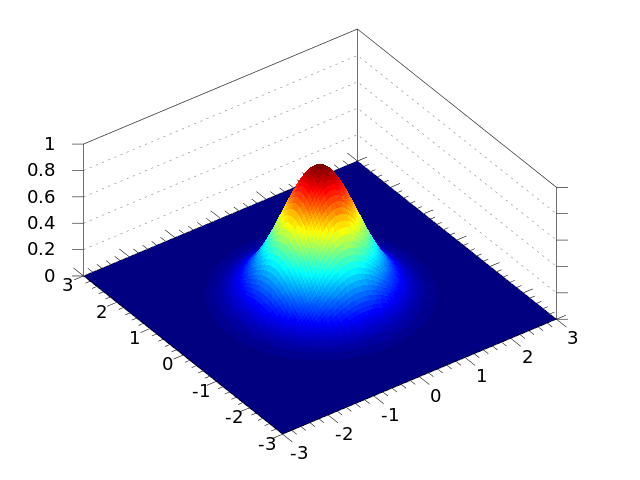
\includegraphics[width=0.6\linewidth]{figs/2d_gaussian}
\end{center}
\begin{easylist}[itemize]
	\ListProperties(Space=\listSpace, Space*=\listSpace)
	# Gaussians arise naturally in sums $x_1 + \dots + x_N$ and averages, since when $N \to \infty$ the sum is normally distributed by the \emph{central limit theorem}.
	# The multidimensional Gaussian can be diagonalized by diagonalizing
	the precision matrix $\vect{\Lambda} = \vect{\Sigma}^{-1}$, then $\exp(\vect{x}^T \vect{\Lambda} \vect{x}) \cong \exp(\vect{y}^T \vect{D} \vect{y})$, where $\vect{D} = \operatorname{diag}(d_1, \dots, d_D)$.
	# One limitation is the unimodal nature of the Gaussian, i.e. it has a single peak.
	
	# \textbf{Partitioned Gaussians.}
	Let $\vect{x} \sim \N (\vect{x} | \vect{\mu}, \vect{\Sigma})$, where $\vect{\Lambda} = \vect{\Sigma}^{-1}$ 
	and 
	\begin{equation*}
	\vect{x} =
	\begin{pmatrix}
	\vect{x}_a \\ 
	\vect{x}_b 
	\end{pmatrix}
	\quad 
	\vect{\mu} =
	\begin{pmatrix}
	\vect{\mu}_a \\ 
	\vect{\mu}_b 
	\end{pmatrix}
	\quad 
	\vect{\Sigma} =
	\begin{pmatrix}
	\vect{\Sigma}_{aa} & \vect{\Sigma}_{ab}  \\ 
	\vect{\Sigma}_{ba} & \vect{\Sigma}_{bb}.\
	\end{pmatrix}.
	\end{equation*}
	## \textbf{Conditional distribution}
	\begin{align*} 
	p(\vect{x}_a |\vect{x}_b )
	&= \N (\vect{x} | \vect{\mu}_{a | b}, \vect{\Lambda}_{aa}^{-1}) \\
	\vect{\mu}_{a | b} &= 
	\vect{\mu}_{a} - \vect{\Lambda}_{aa}^{-1} \vect{\Lambda}_{ab} (\vect{x}_b - \vect{\mu}_b)
	\end{align*}
	
	## \textbf{Marginal distribution}
	\begin{equation*} 
	p(\vect{x}_a  )
	= \N (\vect{x}_a | \vect{\mu}_{a}, \vect{\Sigma}_{aa})
	\end{equation*}
	## These results are proved using inverse of $2 \times 2$ block matrices and examining the quadratic and linear terms in the exponential.
	# There also exist closed-form expressions for Bayes theorem when the prior and likelihood are Gaussians with linear relationship.
\end{easylist}



\subsubsection*{Bayesian interference}
\begin{easylist}[itemize]
	\ListProperties(Space=\listSpace, Space*=\listSpace)
	# Gaussian variables.
	## To estimate $\mu_N$ ($\sigma^2$ is assumed known), use Gaussian prior.
	## To estimate $\lambda = 1/\sigma^2$, use Gamma function as prior, i.e.
	\begin{equation*}
	\operatorname{Gam}(\lambda | a, b) = \frac{b^a \lambda^{a-1}}{\Gamma(a)} \exp (-b \lambda)
	\end{equation*}
	since it has the same functional form as the likelihood.
	# The Student-t distribution may be motivated by:
	## Adding an infinite number of Gaussians with various precisions. 
	## It's the distribution of the sample mean  $(\bar{X} - \mu ) / (S / \sqrt{n})$ when $x_1, \dots, x_N$ are i.d.d. from a Gaussian.
	## As the degrees of freedom $\text{df} \to \infty$, the Student-t distribution converges to a Gaussian.
	An important property of the Student-t distribution is it's \emph{robustness} to outliers.
\end{easylist}

\subsubsection*{Periodic variables}
\begin{easylist}[itemize]
	\ListProperties(Space=\listSpace, Space*=\listSpace)
	# The mean can be measured as $\bar{\theta}$, where we think of the data as lying in a circle.
	# The \emph{von-Mises distribution} is a Gaussian on a periodic domain.
	It is given by
	\begin{equation*}
	p(x | \theta_0, m) = \frac{1}{2 \pi I_0(m)} \exp \left[m \cos (\theta - \theta_0)\right].
	\end{equation*}
\end{easylist}

\subsubsection*{The exponential family}
\begin{easylist}[itemize]
	\ListProperties(Space=\listSpace, Space*=\listSpace)
	# The exponential family is given by
	\begin{equation*}
	p(\vect{x} | \vect{\eta}) =
	g(\vect{\eta})  h (\vect{x}) 
	\exp \left( \vect{\eta}^T u(\vect{x}) \right)
	\end{equation*}
	and many probability functions are members of this family.
	The entries of the vector $\vect{\eta}$ are called \emph{natural parameters}, and $g(\vect{\eta})$ is a normalization constant.
	# Maximum likelihood depends only on the \emph{sufficient statistics} $\sum_n u(\vect{x}_n)$.
	# Non-informative priors make few assumptions,
	letting the data speak for itself.
\end{easylist}

\subsubsection*{Nonparametric methods}
\begin{easylist}[itemize]
	\ListProperties(Space=\listSpace, Space*=\listSpace)
	# The general equation for density estimation is
	\begin{equation*}
	p(\vect{x}) \simeq \frac{K}{NV}
	\end{equation*}
	where $K$ is the number of points in a neighborhood of volume $V$ and $N$ is the total number of points.
	# Kernel functions (or Parzen windows) estimate a neighborhood giving decreasing weight to samples further away, e.g. a Gaussian kernel.
	The volume $V$ is fixed, the data (and kernel function) determines $K$.
	# Nearest neighborhood fixes $K$, letting $V$ be a function of the data.
\end{easylist}

% ----------------------------------------------------------------------------
\subsection{Linear Models for Regression}
\subsection*{Linear basis function models}
\begin{easylist}[itemize]
	\ListProperties(Space=\listSpace, Space*=\listSpace)
	# Estimate the data using a function
	\begin{equation*}
	y(\vect{x}, \vect{w}) = \sum_{j = 0}^{M-1} \vect{w}_j \phi_j(\vect{x}) = \vect{w}^T \vect{\phi}(\vect{x}).
	\end{equation*}
	# The function is linear in $\vect{w}$, but not necessarily in $\vect{x}$ since $\phi_j (\cdot)$ might be non-linear.
	# Choice for the $\phi_j (\cdot)$ include identity, powers of $\vect{x}$, Gaussians, sigmoids, Fourier basis, Wavelet basis, and arbitrary non-linear functions.
	# Assuming a noise term $\epsilon \sim \N(0, \beta^{-1})$, the ML solution $\vect{w}_\text{ML}$ is given by
	\begin{equation*}
	\vect{w}_\text{ML} = \left(\vect{\Phi}^T \vect{\Phi} \right)^{-1} \vect{\Phi}^T \vect{t} = \vect{\Phi}^\dagger \vect{t},
	\end{equation*}
	where $\vect{\Phi}^\dagger$ is the \emph{Moore-Penrose pseudoinverse} and the \emph{design matrix} $\vect{\Phi}$ has entries $\vect{\Phi}_{ij} = \phi_j(\vect{x}_i)$.
	The ML solution is equivalent to minimizing the sum of squares.
	
	# Sequential learning is possible if the gradient descent algorithm is used to compute $\vect{w}^{(\tau + 1)} = \vect{w}^{\tau} - \eta \nabla E_n$.
	This facilitates on-line learning with much data.
	
	# If there are multiple outputs which are linear in the same set of basis functions, the solution is $\vect{w}_k = \vect{\Phi}^\dagger \vect{t}_k$ for every output $k$, i.e. the system decouples.
	
	# Regularizing the error with a quadratic term $\lambda \vect{w}^T \vect{w} /2$ has ML solution by 
	\begin{equation*}
	\left( \alpha \vect{I} + \vect{\Phi}^T \vect{\Phi} \right)
	\vect{w}
	=
	\vect{\Phi}^T \vect{t}.
	\end{equation*}
	The solution above is equivalent to a prior $p(\vect{w} \mid \alpha) = \N (\vect{w} \mid  \vect{0}, \alpha^{-1} \vect{I})$.
\end{easylist}


\subsection*{The Bias-Variance decomposition}
\begin{easylist}[itemize]
	\ListProperties(Space=\listSpace, Space*=\listSpace)
	# The bias-variance decomposition is
	\begin{equation*}
	\text{expected loss} = (\text{bais})^2 + \text{variance} + \text{noise}.
	\end{equation*}
	# Imagine drawing many data sets $\D$.
	## The \textbf{bias} is the distance from the average prediction to the conditional expectation $f(\vect{x}) = \E \left[t | \vect{x} \right]$.
	In other words:
	\begin{equation*}
		\mathrm{Bias}\big[\hat{f}(\vect{x})\big] = \E \big[\hat{f}(\vect{x}) - f(\vect{x})\big]
	\end{equation*}
	## The \textbf{variance} is the variability of $y(\vect{x}; \D)$ around it's average.
	\begin{equation*}
		\mathrm{Var}\big[\hat{f}(\vect{x})\big] = \E [\hat{f}(\vect{x})^2] - \mathrm{E}[{\hat{f}}(\vect{x})]^2
	\end{equation*}
	# Flexible models have high variance, rigid models have high bias.
\end{easylist}

\subsection*{Bayesian linear regression}
\begin{easylist}[itemize]
	\ListProperties(Space=\listSpace, Space*=\listSpace)
	# Introduce a parameter distribution over $\vect{w}$, for instance an isotropic Gaussian distribution with $\vect{S}_0 = \alpha \vect{I}$.
	\begin{equation*}
	p(\vect{w}) = \N (\vect{w} | \vect{m}_0, \vect{S}_0)
	\end{equation*}
	Although the prior $p(\vect{w})$ is isotropic, the posterior $p(\vect{w} \mid \mathsf{t})$ need not be.
	\begin{align*}
	    p(\vect{w}) &= \N ( \vect{w} \mid \vect{m}_0, \vect{S}_0) \quad \tag{prior} \\
	    p(\mathsf{t}\mid \vect{w}) &= \prod_{n=1}^{N} p(t_n \mid \vect{w}) \quad \tag{likelihood} \\
	    p(\vect{w} \mid \mathsf{t}) &= \N ( \vect{w} \mid \vect{m}_N, \vect{S}_N) \quad \tag{posterior} 
	\end{align*}
	
	# Analytical calculations are possible, leading to refinement of the posterior distribution of the parameters $\vect{w}$ as more data is seen.
	
	# A predictive distribution $p(t | \vect{t}, \alpha, \beta)$ can be found.
	The predictive distribution accounts for uncertainty of the parameters $\alpha$ and $\beta$.
	
	# The model may be expressed via an \emph{equivalent kernel} $k(x, x_n)$ as 
	\begin{equation*}
		y(\vect{x}, \vect{w}) =
		y(\vect{x}, \vect{m}_N) =
		\beta \vect{\phi} (\vect{x}) \vect{S}_N \vect{\Phi}^T \mathsf{t}
		=
		\sum_{n=1}^{N} \underbrace{
			\beta \vect{\phi} (\vect{x})^T \vect{S}_N \vect{\phi} (\vect{x}_n)
			}_{k(x, x_n)}
			t_n
	\end{equation*}
	In this context, a kernel is a ``similarity function,'' a dot product in some space.
	This can reduce to lower dimensions and make computations faster.
\end{easylist}

\subsection*{Bayestian model selection and limitations}
\begin{easylist}[itemize]
	\ListProperties(Space=\listSpace, Space*=\listSpace)
	# Bayestian model selection uses Bayes theorem as
	\begin{equation*}
		p( \mathcal{M}_i \mid \D) = \frac{p( \D \mid \mathcal{M}_i) p( \mathcal{M}_i )}{p( \D)}
	\end{equation*}
	where $\mathcal{M}_i$ is a model (distribution).
	It's possible to choose the best model given the data by evaluating the \emph{model evidence} (or \emph{marginal likelihood}) $p( \D \mid \mathcal{M}_i)$ via marginalization over $\vect{w}$.
	
	# Disadvantages of the model considered includes the fact that the functions $\phi_j(\vect{x})$ are fixed before data is observed, and the number of functions often grow exponentially with the number of inputs.
	These shortcomings are often alleviated in other models by the fact that data often lies on a lower-dimensional manifold.
\end{easylist}

% ----------------------------------------------------------------------------
\subsection{Linear Models for Classification}
\begin{easylist}[itemize]
	\ListProperties(Space=\listSpace, Space*=\listSpace, Numbers1=l, FinalMark1={)})
	# sdf
\end{easylist}

% ----------------------------------------------------------------------------
\subsection{Neural networks}
\begin{easylist}[itemize]
	\ListProperties(Space=\listSpace, Space*=\listSpace, Numbers1=l, FinalMark1={)})
	# sdf
\end{easylist}

% ----------------------------------------------------------------------------
\subsection{Kernel methods}
\begin{easylist}[itemize]
	\ListProperties(Space=\listSpace, Space*=\listSpace, Numbers1=l, FinalMark1={)})
	# sdf
\end{easylist}

% ----------------------------------------------------------------------------
\subsection{Sparse Kernel Machines}
\begin{easylist}[itemize]
	\ListProperties(Space=\listSpace, Space*=\listSpace, Numbers1=l, FinalMark1={)})
	# sdf
\end{easylist}

% ----------------------------------------------------------------------------
\subsection{Graphical Models}
\begin{easylist}[itemize]
	\ListProperties(Space=\listSpace, Space*=\listSpace, Numbers1=l, FinalMark1={)})
	# sdf
\end{easylist}

% ----------------------------------------------------------------------------
\subsection{Mixture Models and EM}
\begin{easylist}[itemize]
	\ListProperties(Space=\listSpace, Space*=\listSpace, Numbers1=l, FinalMark1={)})
	# sdf
\end{easylist}

% ----------------------------------------------------------------------------
\subsection{Approximate Interference}
\begin{easylist}[itemize]
	\ListProperties(Space=\listSpace, Space*=\listSpace, Numbers1=l, FinalMark1={)})
	# sdf
\end{easylist}

% ----------------------------------------------------------------------------
\subsection{Sampling Methods}
\begin{easylist}[itemize]
	\ListProperties(Space=\listSpace, Space*=\listSpace, Numbers1=l, FinalMark1={)})
	# sdf
\end{easylist}

% ----------------------------------------------------------------------------
\subsection{Continuous Latent Variables}
\begin{easylist}[itemize]
	\ListProperties(Space=\listSpace, Space*=\listSpace, Numbers1=l, FinalMark1={)})
	# sdf
\end{easylist}

% ----------------------------------------------------------------------------
\subsection{Sequential Data}
\begin{easylist}[itemize]
	\ListProperties(Space=\listSpace, Space*=\listSpace, Numbers1=l, FinalMark1={)})
	# sdf
\end{easylist}

% ----------------------------------------------------------------------------
\subsection{Combining Models}
\begin{easylist}[itemize]
	\ListProperties(Space=\listSpace, Space*=\listSpace, Numbers1=l, FinalMark1={)})
	# sdf
\end{easylist}

% ----------------------------------------------------------------------------
















\clearpage
\section{Exercises}

% ----------------------------------------------------------------------------
\subsection{Introduction}
\subsubsection*{Exercise 1.2}
We start with Equation (1.4) from the book and differentiate it with respect to $w_i$:
\begin{align*}
	\partial_{w_i} \tilde{E}(\vect{w})
	&= \sum_{n=1}^{N} \left[ y(x_n, \vect{w}) - t_n \right] \partial_{w_i} y(x_n, \vect{w}) + \lambda w_i \\
	&= \sum_{n=1}^{N} \left[ y(x_n, \vect{w}) - t_n \right] (x_n)^i + \lambda w_i \\
	&= \sum_{n=1}^{N} \left[ \sum_{j=0}^{M} w_j (x_n)^j - t_n \right] (x_n)^i + \lambda w_i = 0
\end{align*}
Multiplying through the factor $(x_n)^i$ and rearranging the terms yields
\begin{equation*}
	\sum_{j=0}^{M} w_j \underbrace{\sum_{n=1}^{N} (x_n)^{i+j}}_{A_{ij}}
	+
	\lambda w_i = \underbrace{\sum_{n=1}^{N}  (x_n)^i t_n}_{T_{ij}},
\end{equation*}
where the definitions of $A_{ij}$ and $T_{ij}$ are identical to those given in Exercise 1.1.
Finally we employ the Kronecker delta symbol $\delta_{ij}$ to pull the $w_i$ into the sum, since $\lambda w_i = \sum_{j=0}^{M} \lambda \delta_{ij} w_j$ we have
\begin{equation*}
	\sum_{j=0}^{M}  \left( A_{ij} + \delta_{ij} \lambda \right) w_j
	 = T_{ij}.
\end{equation*}
This solves the problem.
Notice that in vector notation this system can be written as 
\begin{equation*}
	\left( \vect{\Phi}^T \vect{\Phi} + \vect{I}\lambda \right) \vect{w} = \vect{\Phi}^T \vect{t},
\end{equation*}
where $\vect{\Phi}_{ij}= (x_i)^j$.
Solving the system solves the regularized polynomial fitting problem.


\subsubsection*{Exercise 1.8}
We first show that $\E \left[x\right] = \mu$.
We define $K(\sigma) = 1 / \sqrt{2 \pi} \sigma$ and evaluate the integral
\begin{align*}
	\E \left[x\right] &= \int K(\sigma) \exp \left( - \frac{1}{2 \sigma^2} \left(x - \mu \right)^2 \right) x \, dx \\
	&= \int K(\sigma) \exp \left( - \frac{1}{2 \sigma^2} z^2 \right) (z + \mu) \, dz \tag{change of variables}\\
	&= \int K(\sigma) \exp \left( - \frac{1}{2 \sigma^2} z^2 \right) z \, dz 
	+
	 \mu \int K(\sigma) \exp \left( - \frac{1}{2 \sigma^2} z^2 \right) \, dz \\
	 & = 0 + \mu,
\end{align*}
where the first integral in the second to last line is zero because it's an odd function integrated over the real line, and the second integral evaluates to $\mu$ since the integrand is unity (it's a centered normal distribution, which has integral $1$).

The second part of the problem asks us to verify that $\E \left[ x^2 \right] = \mu^2 + \sigma^2$.
We factor the normal distribution as $\N\left( x \mid \mu, \sigma^2\right) = K(\sigma^2) E(\sigma^2)$, where
\begin{alignat*}{3}
	& K(\sigma^2) = \left( 2 \pi \sigma^2 \right)^{-1/2} 
	&& \qquad \frac{\partial K}{\partial \sigma^2} = - \left( 2 \pi \sigma^2 \right)^{-3/2} \pi = -K(\sigma^2)^3 \pi \\
	& E(\sigma^2) = \exp \left( - \frac{1}{2 \sigma^2} \left( x - \mu \right)^2 \right)
	&& \qquad \frac{\partial E}{\partial \sigma^2} = \frac{1}{2\sigma^4} \left( x - \mu\right)^2 E(\sigma^2).
\end{alignat*}
We expedite notation by writing these functions as $K$ and $E$, and their derivatives with respect to $\sigma^2$ as $K'$ and $E'$.
Using the product rule of calculus, we have
\begin{gather*}
	\frac{\partial}{\partial \sigma^2} \left( \int K(\sigma^2) E(\sigma^2) \, dx = 1 \right) \\
	\int K' E + K E' \, dx = 0 \\
	\int KE \left( -\pi K^2 + \frac{1}{2 \sigma^4} (x - \mu)^2 \right) \, dx = 0.
\end{gather*}
Substituting $- \pi K^2 = - 1 / (2 \sigma^2)$, expanding the square term, multiplying out the $KE$ term and performing the integrals, we obtain
\begin{equation*}
	-\frac{1}{2\sigma^2} + \frac{1}{2 \sigma^4} \int KE x^2 \, dx + 0 - \frac{\mu^2}{2 \sigma^4} = 0,
\end{equation*}
and solving this for the unknown integral yields $\operatorname{E}\left[x^2\right] = \int KE x^2 \, dx = \mu^2 + \sigma^2$
as required.

To show that Equation (1.51) from the book holds, notice that
\begin{align*}
	\var \left[ x \right] &= \E\left[ (x - \E\left[x\right])^2\right] 
	= \E\left[ x^2 - 2 x \mu + \mu ^2\right] \\
	&= \E\left[ x^2\right] - 2 \mu^2 + \mu^2 
	= \E\left[ x^2\right] - \E\left[ x\right]^2,
\end{align*}
where we have used $\mu$ interchangeably with $\E\left[ x\right]$. 



\subsubsection*{Exercise 1.10}
Recall that the definition of the expected value is
$\E\left[x\right] = \int p(x) x \, dx$, and that $\int p(x) \, dx = 1$
Statistical independence means that $p(x, y)$ factors as $p(x)p(y)$, so we have
\begin{align*}
	\E\left[x + y\right] &= \iint p(x, y) (x+y) \, dx \, dy 
	= \iint p(x) p(y) (x+y) \, dx \, dy \tag{independence} \\
	&= \iint p(x) p(y) x \, dx \, dy + \iint p(x) p(y) y \, dx \, dy \\
	&= \int p(y) \left( \int  p(x)  x \, dx \right) \, dy + \int p(y) y \left( \int p(x)  \, dx \right) \, dy \\
	&= \int p(y) \left( \E \left[ x \right] \right) \, dy + \int p(y) y \, dy \tag{by definition} 
	= \E\left[x\right] + \E\left[y\right]
\end{align*}

To show that $\var\left[x + y\right] = \var\left[x\right] + \var\left[y\right]$, we use the preceding result along with the definition from Equation (1.38) in \cite{bishop_pattern_2011}  $\var\left[x\right] = \E\left[ (x - \E\left[x\right])^2\right]$ to write
\begin{align*}
	\var\left[x + y\right] &= \E\left[ \left( (x + y) - \E \left[ x + y \right] \right)^2\right] \\
	&= \E\left[ \left( \left(x - \E\left[x\right]\right) + \left(y - \E\left[y\right]\right) \right)^2\right] \tag{rearranging} \\
	&= \E\left[  \left(x - \E\left[x\right]\right)^2 + 2 \left(x - \E\left[x\right]\right) \left(y - \E\left[y\right]\right) + \left(y - \E\left[y\right]\right)^2\right] \\
	&= \E\left[  \left(x - \E\left[x\right]\right)^2 \right]
	+
	\underbrace{\E\left[   2 \left(x - \E\left[x\right]\right) \left(y - \E\left[y\right]\right) \right]}_{0}
	+
	\E\left[   \left(y - \E\left[y\right]\right)^2\right] \\
	&= \var\left[x\right] + \var\left[y\right].
\end{align*}
The cross term vanishes since $x$ and $y$ are independent.
We will not show this in detail, but it can be shown by first noticing that $\E \left[xy\right] = \E \left[x\right] \E \left[y\right]$ when $x$ and $y$ are independent, and then showing that $\E\left[    \left(x - \E\left[x\right]\right) \right] = \E\left[ x \right] - \E\left[ x \right] = 0$.

\subsubsection*{Exercise 1.15}
Due to the size of this problem, we split the solution into parts.
\begin{easylist}[enumerate]
	\ListProperties(Space=\listSpace, Space*=\listSpace, Numbers1=l, FinalMark1={)})
	# The redundancy is present due to the fact fact multiplication is commutative, so the weights may be factored out.
	For instance, when $M=2$, we see that 
	\begin{equation*}
		w_{ij}x_i x_j + w_{ji} x_j x_i = (w_{ij} + w_{ji}) x_i x_j = \widetilde{w}_{ij} x_i x_j.
	\end{equation*}
	We remove redundancy by ordering the products in a common term with $i_1 \geq i_2 \geq \cdots \geq i_M$.
	This ordering corresponds to Equation (1.134).
	
	For instance, instead of summing over terms with $x_1 x_2 x_3$, $x_1 x_3 x_2$, $x_2 x_1 x_3$ and so forth, we make use of a common weight for the $x_3 x_2 x_1$-term.
	
	# The total number of terms equals the number of terms in the nested sum
	\begin{equation*}
		n(D, M) = \sum_{i_1 = 1}^{D} 
		\sum_{i_2 = 1}^{i_1}
		\cdots
		\sum_{i_M = 1}^{i_{M - 1}} 1,
	\end{equation*}
	which contains $M$ sums.
	To prove the recursive formula, we expand the outer sum and notice that the result is $D$ nested sums over $M-1$ sums each.
	We have
	\begin{align*}
		n(D, M) &= \sum_{i_1 = 1}^{D} 
		\sum_{i_2 = 1}^{i_1}
		\cdots
		\sum_{i_M = 1}^{i_{M - 1}} 1 \\
		&= 
		\left( 
		\sum_{i_2 = 1}^{1}
		\cdots
		\sum_{i_M = 1}^{i_{M - 1}} 1
		\right)+\left( 
		\sum_{i_2 = 1}^{2}
		\cdots
		\sum_{i_M = 1}^{i_{M - 1}} 1
		\right)+
		\cdots
		+\left( 
		\sum_{i_2 = 1}^{D}
		\cdots
		\sum_{i_M = 1}^{i_{M - 1}} 1 \right) \\
		&= n(D=1, M-1) + n(D=2, M-1) + \cdots + n(D=D, M-1) \\
		&= \sum_{i=1}^{D} n(i, M-1).
	\end{align*}
	
	# We skip the base case, which is easily verified.
	Assuming the result holds for $D$, we we show that it holds for $D+1$ by writing
	\begin{align*}
		\sum_{i=1}^{D + 1} \frac{(i +M - 2)!}{(i-1)!\, (M-1)!} &=
		\sum_{i=1}^{D} \frac{(i +M - 2)!}{(i-1)! \, (M-1)!}
		+  \frac{(D+M-1)!}{D! \, (M-1)!}.
	\end{align*}
	The sum on the right hand side is the given result for $D$, which we assume is true.
	Substituting this fact, we write
	\begin{align*}
		\sum_{i=1}^{D + 1} \frac{(i +M - 2)!}{(i-1)! \, (M-1)!} &=
		\frac{(D + M - 1)!}{(D- 1)! \, M!}
		+  \frac{(D+M-1)!}{D! \, (M-1)!} \\
		&=
		\frac{(D + M - 1)! \, D}{D! \, M!}
		+  \frac{(D+M-1)! \, M}{D! \, M!} \\
		&=
		\frac{(D + M - 1)! \, (D + M)}{D! \, M!} = \frac{(D + M)!}{D!\, M!} \\
		&=\frac{((D+1) + M - 1)!}{((D+1) - 1)! \, M!},
	\end{align*}
	which shows that the result holds for $D+1$ when it holds for $D$.
	
	# We skip the base case of the inductive argument, as it should be easy to carry out.
	
	The inductive step is performed as follows.
	Below, the first equality comes from Equation (1.135) in the book,
	the second comes from assuming the result holds for $M-1$,
	and the third comes from Equation (1.136).
	\begin{equation*}
		n(D, M) = \sum_{i=1}^{D} n(i, M - 1)
		= \sum_{i=1}^{D} \frac{(i +M - 2)!}{(i-1)!\, (M-1)!} 
		= 
		 \frac{(D + M - 1)!}{(D - 1)! \, M !}.
	\end{equation*}
	Comparing the first and final expression, we observe that if we assume the relation holds for $M-1$, it does indeed hold for $M$ too.
\end{easylist}


\subsubsection*{Exercise 1.21}
Starting with the inequality $a \leq b$, we multiply both sides by $a > 0$ to obtain $a^2 \leq ab$.
We can take the square root of both sides and preserve the inequality, since the square root is monotonically increasing.
Doing so, we obtain the desired inequality.

To prove the integral inequality, we apply the inequality on each term in Equation (1.78), then replace the integral over $\mathcal{R}_1 \cup \mathcal{R}_2$ with the real line:
\begin{align*}
	p(\text{mistake}) &= \int_{\mathcal{R}_1} p(\vect{x}, \mathcal{C}_2) \, d 
	\vect{x}
	+
	\int_{\mathcal{R}_2} p(\vect{x}, \mathcal{C}_1) \, d \vect{x} \\
	&\leq 
	 \int_{\mathcal{R}_1} \left\{ p(\vect{x}, \mathcal{C}_1) \, p(\vect{x}, \mathcal{C}_2) \right\}^{1/2} \, d \vect{x}
	+
	\int_{\mathcal{R}_2} \left\{ p(\vect{x}, \mathcal{C}_2) 
	\, p(\vect{x}, \mathcal{C}_1) \right\}^{1/2} \, d \vect{x} \\
	&= \int \left\{ p(\vect{x}, \mathcal{C}_2) \, p(\vect{x}, \mathcal{C}_1) \right\}^{1/2} \, d \vect{x}
\end{align*}

\subsubsection*{Exercise 1.25}
This closely follows the derivation in Section 1.5.5.
If $\vect{x} \in \R^n$ and $\vect{t} \in \R^m$, we view
$\E \left[L (\vect{t}, \vect{y} (\vect{x}))\right]$ as a functional from the set of functions $\{ f \mid f: \R^n \to \R^m \}$ to $\R$.
Comparing the ordinary derivative and the functional derivative, we see that
\begin{align*}
	f(\vect{x} + \vect{\epsilon}) &= f(\vect{x}) 
	+
	\vect{\epsilon}^T \nabla f(\vect{x}), \quad \text{and}
	\\
	F(\vect{y}(\vect{x}) + \epsilon \vect{\eta}(\vect{x})) &=
	F(\vect{y}(\vect{x})) + \epsilon \int \int  \vect{\eta}^T
	\delta_{\vect{y}_j(\vect{x})} F(\vect{y}(\vect{x}))
	  \, d \vect{t} \, d\vect{x} \\
	&=
	 F(\vect{y}(\vect{x}))
	+
	\epsilon \sum_{j=1}^{n}
	 \int \underbrace{\left( \int \frac{\delta F(\vect{y}(\vect{x}))}{\delta \vect{y}_j(\vect{x})} \, d \vect{t} \right)}_{\text{must be } 0} \eta_j (\vect{x}) \, d \vect{x}.
\end{align*}
The above condition implies that
\begin{equation*}
	\left( \int \frac{\delta F(\vect{y}(\vect{x}))}{\delta \vect{y}_j(\vect{x})} \, d \vect{t} \right)=
	2 \int ( \vect{y}_j(\vect{x}) - \vect{t}_j) p (\vect{x}, \vect{t}) \, d\vect{t}
	= 0,
\end{equation*}
which, following the derivation leading to Equation (1.89), leads to
\begin{equation*}
	\vect{y}_j(\vect{x}) = \int t_j p (\vect{t} \mid \vect{x}) \, d \vect{t} = \E_{\vect{t}} \left[ t_j \mid \vect{x} \right].
\end{equation*}
This applies to any  component $j$ of $\vect{y}(\vect{x})$, so $\vect{y}(\vect{x}) = \E_{\vect{t}} \left[ \vect{t} \mid \vect{x} \right]$.
To show that this reduces to Equation (1.89) in the case of a single target variable, simply define $\vect{t} := (t)$, i.e. a vector with one component.




\subsubsection*{Exercise 1.33}
A hint as to why this is true is given on page 54, which states that $\H\left[y 
\mid x\right]$ is ``the average additional information needed to specify $y$, 
given $x$.''
If the conditional entropy is zero, then $y$ must be completely specified by $x$, i.e. a function of $x$.
If $\H\left[y \mid x\right] = 0$, then
\begin{equation*}
	\sum_i \sum_j p(x_i, y_j) \ln p (y_j \mid x_i) = 0.
\end{equation*}
Using $ p(x_i, y_j) = p(y_j \mid x_i) p(x_i)$ and rearranging the sums, we obtain
\begin{equation*}
	\sum_i p(x_i) \left[ \sum_j p(y_j \mid x_i)  \ln p (y_j \mid x_i) \right] = 0.
\end{equation*}
We know that $0 \leq p (x_i) \leq 1$ for every $x_i$.
Assuming now that $p (x_i) > 0$, the bracketed term must be zero for every $i$, i.e.
\begin{equation*}
	\sum_j p(y_j \mid x_i)  \ln p (y_j \mid x_i) = 0 \quad \text{for every } i.
\end{equation*}
Consider now the term $p(y_j \mid x_i)  \ln p (y_j \mid x_i)$.
The functional form of this term is $z \ln z$, and this function is negative 
except when $z = 0$ and when $z=1$, where it is zero.
Since we are adding terms that are either negative or zero, and the sum must 
evaluate to zero, every term in the sum must be zero.
Therefore, $p(y_j \mid x_i)$ must be 0 or 1 for each value of $y_j$.
However, since $\sum_j p(y_j \mid x_i) = 1$, every value of $p(y_j \mid x_i)$ 
must be zero except for one.
In other words, $x_i$ completely determines $y_j$.


\subsubsection*{Exercise 1.38}
We wish to prove Equation (1.115) based on Equation (1.114).
Clearly the case $M=1$ is true, and we assume the case $M=2$ is true, since this is given by Equation (1.114).
For the inductive step, we assume the identity holds in the base case, and in 
the $M-1$ case, and then
\begin{align*}
	f \left( \sum_{i=1}^{M} \lambda_i x_i \right)
	&= f \left( \sum_{i=1}^{M-1} \lambda_i x_i + \lambda_M x_M \right)
	= f \left( \frac{\sum_{k=1}^{M-1} \lambda_k}{\sum_{k=1}^{M-1} \lambda_k} \sum_{i=1}^{M-1} \lambda_i x_i + \lambda_M x_M \right).
\end{align*}
The sum of $\sum_{k=1}^{M-1} \lambda_k$ and $\lambda_M$ is unity, and $\sum_{i=1}^{M-1} \lambda_i x_i / \sum_{k=1}^{M-1} \lambda_k$ is a weighted average of $x$-values.
Since it's a weighted average, it may be treated as just another $x$-value.

Applying the base case for two $x$ values, we obtain
\begin{equation*}
	f \left( \frac{\sum_{k=1}^{M-1} \lambda_k}{\sum_{k=1}^{M-1} \lambda_k} \sum_{i=1}^{M-1} \lambda_i x_i + \lambda_M x_M \right)
	\leq
	\left( \sum_{k=1}^{M-1} \lambda_k \right) f \left( 
	\frac{1}{\sum_{k=1}^{M-1} \lambda_k} \sum_{i=1}^{M-1} \lambda_i x_i
	 \right)
	+
	\lambda_M f \left( x_M \right).
\end{equation*}
Now we can appeal to the $M-1$ case of the inequality, which we assume to be true by the induction hypothesis.
We can appeal to it since the $\lambda_i / \sum_{k=1}^{M-1} \lambda_k$ are normalized and sum to unity in the equation above due to the normalizing factor in front of the sum.
To ease notation, we define $\alpha = \sum_{k=1}^{M-1} \lambda_k$ and write
\begin{equation*}
\alpha f \left( 
 \sum_{i=1}^{M-1} \frac{\lambda_i}{\alpha} x_i
\right)
+
\lambda_M f \left( x_M \right)
\leq
\alpha \left( \sum_{i=1}^{M-1} \frac{\lambda_i}{\alpha} f(x_i) \right)
+
\lambda_M f \left( x_M \right)
=
\sum_{i=1}^{M} \lambda_i f(x_i).
\end{equation*}
This proves the Jensen inequality.


% ----------------------------------------------------------------------------
\subsection{Probability Distributions}
\subsubsection*{Exercise 2.6}
We split this problem into three parts: the (a) expected value, (b) variance and (c) mode.
\begin{easylist}[enumerate]
	\ListProperties(Space=\listSpace, Space*=\listSpace, Numbers1=l, FinalMark1={)})
	# The \textbf{expected value} is computed from the definition as
	\begin{align*}
		\E[\mu] &= \int \mu p(\mu) \, d\mu =  \frac{\Gamma(a + b)}{\Gamma(a ) \Gamma( b)} \int_0^a \mu \, \mu^{a-1} (1- \mu)^{b-1} \, d\mu \\
		&= \frac{\Gamma(a + b)}{\Gamma(a ) \Gamma( b)} \int_0^a  \mu^{(a+1)-1} (1- \mu)^{b-1} \, d\mu \tag{re-cast as Beta} \\ 
		&= \frac{\Gamma(a + b)}{\Gamma(a ) \Gamma( b)} \frac{\Gamma(a +1 ) \Gamma( b)}{\Gamma(a + b + 1)} = \frac{a}{a + b},
	\end{align*}
	where we used Equation (2.265) from \cite{bishop_pattern_2011}, along with $\Gamma(x+1) = x\Gamma(x)$.
	
	# To compute the \textbf{variance}, we will employ $\var[\mu] = \E[\mu^2] - \E[\mu]^2$.
	Similarly to the sub-problem above, we observe that
	\begin{align*}
	\E[\mu^2] &= \frac{\Gamma(a + b)}{\Gamma(a ) \Gamma( b)} \int_0^a  \mu^{(a+2)-1} (1- \mu)^{b-1} \, d\mu \\
	&= \frac{\Gamma(a + b)}{\Gamma(a ) \Gamma( b)} \frac{\Gamma(a +2 ) \Gamma( b)}{\Gamma(a + b + 2)}
	= \frac{(a+1) a}{(a + b +1) (a+b)},
	\end{align*}
	where in the last equality we have used $\Gamma(x+2) = (x+1)x \Gamma(x)$, which is simply repeated application of $\Gamma(x+1) = x\Gamma(x)$ twice.
	
	At this point, we're left with
	\begin{equation*}
		\var[\mu] = \E[\mu^2] - \E[\mu]^2 = \frac{(a+1) a}{(a + b +1) (a+b)} - \left( \frac{a}{a + b} \right),
	\end{equation*}
	which after some manipulation equals the desired result.
	We omit the details.
	
	# The \textbf{mode} is the maximum of the distribution.
	We differentiate the p.d.f. using the product rule of calculus to obtain
	\begin{equation*}
		p'(\mu) = (a-1) \mu{a-2} (1-\mu)^{b-1}
		+
		\mu^{a-1} (b-1) (1-\mu)^{b-2}(-1) = 0.
	\end{equation*}
	Diving by $\mu^a$ and $(1-\mu)^b$ and rearranging, we obtain
	\begin{equation*}
		\frac{(a-1)}{(b-1)} \frac{(1 - \mu)}{\mu} = 1.
	\end{equation*}
	Solving the equation above for $\mu$ yields  $(a-1) / (a + b - 2)$ as required.
\end{easylist}

\subsubsection*{Exercise 2.8}
The \textbf{first part} is to show Equation (2.270). 
We apply the definitions of $E_x \left[ x \mid y \right]$ and $E_y [f(y)]$ in turn, and then the product rule of probability.
Doing so, we have
\begin{align*}
	E_y \left[ E_x \left[ x \mid y \right]  \right] &= 
	E_y \left[ \int x p (x \mid y) \, dx  \right] 
	= \int \left( \int x p (x \mid y) \, dx \right)  p(y) \, dy \\
	&=  \iint x p(x, y) \, dx \, dy = \E[x].
\end{align*}

The \textbf{second part}, which consists of proving Equation (2.271), is slightly more involved.
It helps to keep track of whether the quantities are constants, functions of $x$ or functions of $y$.
It's also useful to know, from the definition of conditional variance, that
\begin{equation}
\label{eqn:conditional_variance}
	\var_x[ x \mid y ] 
	=
	\int p(x \mid y) \left( x - E_x \left[ x \mid y \right] \right)^2 \, dx
	=
	 \E_x [x^2 \mid y] - \E_x [x \mid y]^2.
\end{equation}
The result above does not come as a surprise, since it's merely the familiar result for variance, i.e. $\var_x[ x ] = \E_x [x^2] - \E_x [x ]^2$, conditioned on $y$ in every term.

Let's examine the \textbf{first term} in the right hand side of (2.270) first, i.e. $\E_y \left[ \var_x[ x \mid y ]  \right]$.
Using equation \eqref{eqn:conditional_variance} above, we see that
\begin{align}
	\nonumber \E_y \left[ \var_x[ x \mid y ]  \right] &=  \E_y \left[ \E_x [x^2 \mid y] - \E_x [x \mid y]^2  \right]
	=
	\E_y \left[ \E_x [x^2 \mid y] \right] - \E_y \left[ \E_x [x \mid y]^2  \right] \\
	\label{eqn:ch2_prob8a} &= \E[x^2] - \E_y \left[ \E_x [x \mid y]^2  \right],
\end{align}
where we used Equation (2.270) from the book in the last equality.

We now investigate the \textbf{second term} in Eqn (2.270), i.e. 
$\var_y \left[ \E_x \left[ x \mid y \right] \right]$.
Using the definition of variance (Equation (1.38) in \cite{bishop_pattern_2011}), followed by Equation (2.270) from the book, and the linearity of the expected value, we obtain
\begin{align}
\nonumber \var_y \left[ \E_x \left[ x \mid y \right] \right]
&= \E_y \left[ 
\left( \underbrace{\E_x \left[ x \mid y \right]}_{f(y)} - 
\underbrace{\E_y \left[ \E_x \left[ x \mid y \right] \right]}_{\text{scalar}} 
\right)^2 \right]   \\
\nonumber &= \E_y \left[ 
\left( \E_x \left[ x \mid y \right] - 
\E[x]
\right)^2 \right] \tag{previous result} \\
\nonumber &= \E_y \left[ 
\E_x \left[ x \mid y \right]^2
-2 \E_x \left[ x \mid y \right] \E[x]
+\E[x]^2
\right] \tag{multiply} \\
\nonumber &= \E_y \left[ 
\E_x \left[ x \mid y \right]^2 \right]
-\E_y \left[ 2 \E_x \left[ x \mid y \right] \E[x] \right]
+\E_y \left[ \E[x]^2
\right] \tag{linearity} \\
 \nonumber &= \E_y \left[ 
\E_x \left[ x \mid y \right]^2 \right]
- 2 \E_y \left[ \E_x \left[ x \mid y \right] \right] \E[x] 
+ \E[x]^2
 \tag{constants}\\
\label{eqn:ch2_prob8b} &= \E_y \left[ 
 \E_x \left[ x \mid y \right]^2 \right]
 - \E[x]^2
\end{align}
Finally, adding Equations \eqref{eqn:ch2_prob8a} and \eqref{eqn:ch2_prob8b} gives the result we're after.


\subsubsection*{Exercise 2.15}
The entropy is given by $\H[p(\vect{x})] = - \int p(\vect{x}) \ln p(\vect{x}) \, d\vect{x}$, and we start by computing the logarithm of $p(\vect{x})$, which is
\begin{equation*}
	\ln p(\vect{x}) = -\frac{D}{2} \ln (2 \pi ) - \frac{1}{2} \ln \abs{\vect{\Sigma}} - \frac{1}{2} (\vect{x} - \vect{\mu})^T \vect{\Sigma}^{-1}(\vect{x} - \vect{\mu}).
\end{equation*}
Defining $\Delta^2$ as $(\vect{x} - \vect{\mu})^T \vect{\Sigma}^{-1}(\vect{x} - \vect{\mu})$ (see Equation (2.44) in the book), we have
\begin{equation*}
	\H[p(\vect{x})] = - \int p(\vect{x}) \ln p(\vect{x}) \, d\vect{x} = 
	\frac{D}{2} \ln (2 \pi ) + \frac{1}{2} \ln \abs{\vect{\Sigma}}
	+ \frac{1}{2}\int   p(\vect{x}) \Delta^2 \, d\vect{x},
\end{equation*}
since $\int K p(\vect{x}) \, d\vect{x} = K$ for constants $K$ such as $D \ln (2\pi) /2$.
The only troublesome term is the last one, so what remains to do is show that $\int p(\vect{x}) \Delta^2 \, d\vect{x} = D$.
If we can show this, then we've proven the equation given in the problem statement.

We will now show that $\int p(\vect{x}) \Delta^2 \, d\vect{x} = D$.
First, however, we'll present a result for the univariate Gaussian, which we will need later on. 
Here's the univariate result, easily proved using partial integration.
\begin{equation}
\label{eqn:ch2_problem15_a}
	\frac{1}{\sqrt{2 \pi} \sigma} \int \exp \left( - \frac{x^2}{2 \sigma^2}\right) \, dx = 
	\frac{1}{\sqrt{2 \pi} \sigma} \int \frac{x^2}{\sigma^2} \exp \left( - \frac{x^2}{2 \sigma^2}\right) \, dx = 1
\end{equation}

%then we'll rotate into eigenvector space by a change of variables $\vect{y} = \vect{U}(\vect{x} - \vect{\mu})$ and evaluate the integral.

We now rotate into $\vect{y}$-space by $\vect{y} = \vect{U}(\vect{x} - \vect{\mu})$, which diagonalizes $\vect{\Sigma}^{-1}$.
From Equations (2.50) and (2.56) in \cite{bishop_pattern_2011}, we see that the integral $\int \Delta^2  p(\vect{x}) \, d\vect{x}$ now becomes
\begin{align*}
	\int_{\R^D} \left( \sum_{i=1}^{D} \frac{y_i^2}{\lambda_i} \right)
	\prod_{j=1}^{D} \frac{1}{(2 \pi \lambda_j)^{1/2}} 
	\exp \left( - \frac{y_j^2}{2 \lambda_j} \right) \, d \vect{y}.
\end{align*}
Multiplying the product into the sum, and integrating each term, we have
\begin{align*}
\sum_{i=1}^{D} \int_{\R^D}  \frac{y_i^2}{\lambda_i} 
\prod_{j=1}^{D} \frac{1}{(2 \pi \lambda_j)^{1/2}} 
\exp \left( - \frac{y_j^2}{2 \lambda_j} \right)  \, d \vect{y},
\end{align*}
where $d \vect{y} := d y_1 \, d y_2 \, \cdots \, d y_D$.
To clarify the meaning of the above equation, let's focus on term $i$ in the outer sum and write out the products more explicitly, the above integral is
\begin{equation}
\label{eqn:ch2_problem15_b}
	\left( \int \frac{1}{(2 \pi \lambda_1)^{1/2}} \exp \left( - \frac{y_1^2}{2 \lambda_1} \right) \, d y_1 \right)
	\cdots
	%\left( \int \frac{1}{(2 \pi \lambda_j)^{1/2}} \exp \left( - \frac{y_j^2}{2 \lambda_1} \right) \, d y_j \right)
	\left( \int \frac{1}{(2 \pi \lambda_D)^{1/2}} \exp \left( - \frac{y_D^2}{2 \lambda_D} \right) \, d y_D \right),
\end{equation}
but the $i$th factor is special, since it has the additional $y_i^2 / \lambda_i$ factor, i.e. it's given by
\begin{equation}
\label{eqn:ch2_problem15_c}
	\left( \int \frac{1}{(2 \pi \lambda_i)^{1/2}} \frac{y_i^2}{\lambda_i}   \exp \left( - \frac{y_i^2}{2 \lambda_i} \right) \, d y_i \right).
\end{equation}
Now comes the crucial observation; every factor in \eqref{eqn:ch2_problem15_b} except the $i$th is a univariate Gaussian, so these integrals evaluate to 1.
The special $i$th term \eqref{eqn:ch2_problem15_c} is in same functional form as \eqref{eqn:ch2_problem15_a} (with $\lambda_i = \sigma^2$), so it also evaluates to 1.
Therefore the product of integrals for every term $i$ evaluates to a product of ones, and the sum is simply
\begin{align*}
\sum_{i=1}^{D} \int_{\R^D}  \frac{y_i^2}{\lambda_i} 
\prod_{j=1}^{D} \frac{1}{(2 \pi \lambda_j)^{1/2}} 
\exp \left( - \frac{y_j^2}{2 \lambda_j} \right)  \, d \vect{y}
=
\sum_{i=1}^{D} 1 = D.
\end{align*}
We've shown that $\int p(\vect{x}) \Delta^2 \, d\vect{x} = D$, and this solves the problem.

\subsubsection*{Exercise 2.20}
We expand $\vect{a}$ in the eigenvector basis of $\vect{\Sigma}$, writing $\vect{a} = \sum_i \alpha_i \vect{u}_i$.
Using the fact that $\vect{u}_i \vect{u}_j = \delta_{ij}$, we have
\begin{align*}
	\vect{a}^T \vect{\Sigma} \vect{a} 
	&= \vect{a}^T \vect{\Sigma} \sum_i \alpha_i \vect{u}_i
	= \vect{a}^T \sum_i \alpha_i \vect{\Sigma} \vect{u}_i
	= \vect{a}^T \sum_i \alpha_i \lambda_i \vect{u}_i \\
	&= \sum_j \alpha_j \vect{u}^T_j \sum_i \alpha_i \lambda_i \vect{u}_i
	= \sum_i \alpha_i^2 \lambda_i.
\end{align*}
If $\lambda_i > 0$ for every $i$, then clearly the sum is positive---so it's sufficient.
On the other hand, if the sum is positive, then no $\lambda_i$ can be negative or zero.
If it were, we could choose $\vect{a}$ in the direction of the corresponding eigenvector and obtain a negative sum, which would be a contradiction.
In other words, it's a also necessary condition that $\lambda_i > 0$ for every $i$.


\subsubsection*{Exercise 2.27}
We split this exercise into two parts.
\begin{easylist}[enumerate]
	\ListProperties(Space=\listSpace, Space*=\listSpace, Numbers1=l, FinalMark1={)})
	# We wish to show that $\E[\vect{x} + \vect{z}] = \E[\vect{x}] + \E[ \vect{z}]$.
	 Using the definition of the expected value, along with independence, we see that
	\begin{align*}
		\E[\vect{x} + \vect{z}] &= \iint (\vect{x} + \vect{z}) p(\vect{x}, \vect{z}) \, d\vect{x} \, d\vect{z} 
		= \iint (\vect{x} + \vect{z}) p(\vect{x}) p(\vect{z}) \, d\vect{x} \, d\vect{z}\\
		&= \int \vect{x} p(\vect{x}) p(\vect{z}) \, d\vect{x} \, d\vect{z} + \int \vect{z} p(\vect{x}) p(\vect{z}) \, d\vect{x} \, d\vect{z}
		= \E[\vect{x}] + \E[ \vect{z}].
	\end{align*}
	
	# As in the previous sub-problem, we use the definition to obtain
	\begin{align*}
	\cov[\vect{x} + \vect{z}] &= \E \left[ (\vect{x} + \vect{z} - \E[\vect{x} + \vect{z}]) (\vect{x} + \vect{z} - \E[\vect{x} + \vect{z}])^T \right] \\
	&= \E \left[ (\vect{x} - \E[\vect{x}] + \vect{z} - \E[\vect{z}]) (\vect{x} - \E[\vect{x}] + \vect{z} - \E[\vect{z}])^T \right].
	\end{align*}
	We wish to expand the inner square term.
	In order to avoid too heavy notation, we introduce $\vect{a}:= \vect{x} - \E[\vect{x}]$ and $\vect{b} := \vect{z} - \E[\vect{z}]$.
	From there, we observe that
	\begin{align*}
	\E \left[ (\vect{a} + \vect{b}) (\vect{a} + \vect{b})^T \right] = \E \left[ \vect{a}\vect{a}^T + \vect{a}\vect{b}^T + \vect{b}\vect{a}^T + \vect{b}\vect{b}^T \right]
	=
	\E \left[ \vect{a}\vect{a}^T  \right] +
	2 \E \left[ \vect{a}\vect{b}^T  \right] +
	\E \left[  \vect{b}\vect{b}^T \right].
	\end{align*}
	Using the definitions of $\vect{a}$ and $\vect{b}$, we see that this is
	\begin{equation*}
		\cov[\vect{x}] + 2 \cov[\vect{x}, \vect{z}] + \cov[\vect{z}],
	\end{equation*}
	and since the variables are independent,  $\cov[\vect{x}, \vect{z}] = \vect{0}.$
	We have shown that 
	\begin{equation*}
		\cov[\vect{x} + \vect{z}] = \cov[\vect{x}] + \cov[\vect{z}].
	\end{equation*}
\end{easylist}

\subsubsection*{Exercise 2.31}
If $y = x + z$, then $p_y(y) = p_x(x) * p_z(z)$, where $*$ denotes the \emph{convolution}.
To see why this is true, draw an $x$-$z$ coordinate system and sketch a line $x + z = a$.
The probability that $y = x + z = a$ is $p_y(y=a) = \int p_x(a - t) p_z(a) \, dt$, since this sums over all possible ways to obtain the sum $a$.

In this case, when have $\vect{y} = \vect{x} + \vect{z}$, so we evaluate
\begin{align*}
	p_y(\vect{y}) &= p_x(\vect{x}) * p_z(\vect{z}) = 
	\int p_x(\vect{y} - \vect{t}) p_z(\vect{y}) \, d \vect{t} \\
	&=
	\int 
	\underbrace{\N \left( \vect{y} \mid \vect{\mu}_{\vect{x}} + \vect{t} , \vect{\Sigma}_{\vect{x}} \right) }_{p(\vect{y} \mid \vect{t})}
	\underbrace{\N \left( \vect{t} \mid \vect{\mu}_{\vect{z}} , \vect{\Sigma}_{\vect{z}} \right)}_{p(\vect{t})}
	 \, d \vect{t}.
\end{align*}
Matching terms with Equations (2.109) and (2.110) we see that
\begin{equation*}
	p_y(\vect{y}) = \N \left( \vect{y} \mid 
	\vect{\mu}_{\vect{z}} + \vect{\mu}_{\vect{x}}
	, \vect{\Sigma}_{\vect{z}} + \vect{\Sigma}_{\vect{x}} \right).
\end{equation*}


\subsubsection*{Exercise 2.40}
The posterior is proportional to the prior times the likelihood, i.e.
\begin{align*}
	p( \vect{\mu} \mid \vect{X} ) &\propto p(\vect{\mu}) p (\vect{X} \mid \vect{\mu}) 
	= \N \left( \vect{\mu} \mid \vect{\mu}_0, \vect{\Sigma}_0 \right)
	\prod_{n=1}^{N}
	\N \left( \vect{x} \mid \vect{\mu}, \vect{\Sigma} \right).
\end{align*}
We ignore normalization constants and only consider the product of the exponential functions, this approach yields
\begin{align}
	\nonumber p( \vect{\mu} \mid \vect{X} ) & \propto \N \left( \vect{\mu} \mid \vect{\mu}_N, \vect{\Sigma}_N \right) \\
	\label{eqn:ch2_prob40_a} &= \exp\left( - \frac{1}{2} \left( 
	(\vect{\mu} - \vect{\mu}_0)^T \vect{\Sigma}_0^{-1} (\vect{\mu} - \vect{\mu}_0)
	+
	\sum_{n=1}^{N} (\vect{x}_n - \vect{\mu})^T \vect{\Sigma}^{-1} (x_n - \vect{\mu})
	 \right) \right).
\end{align}
We will multiply out the quadratic forms, and compare it to
\begin{equation}
\label{eqn:ch2_prob40_b}
	(\vect{\mu} - \vect{\mu}_N)^T \vect{\Sigma}_N^{-1} (\vect{\mu} - \vect{\mu}_N)
	= \vect{\mu}^T \vect{\Sigma}_N^{-1} \vect{\mu} - 2 \vect{\mu}_N^T \vect{\Sigma}_N^{-1} \vect{\mu} + \text{const}.
\end{equation}
Multiplying out the terms in the inner parenthesis of Equation \eqref{eqn:ch2_prob40_a} and rearranging, we obtain the expression
\begin{align*}
	\vect{\mu}^T \left( \vect{\Sigma}_0^{-1} + N \vect{\Sigma}^{-1} \right) \vect{\mu} - 2 
	\left( \vect{\mu}_0^T \vect{\Sigma}_0^{-1} + N \vect{\mu}_{\text{ML}}^T  \vect{\Sigma}^{-1} \right) \vect{\mu} + \text{const}.
\end{align*}
Comparing the above with \eqref{eqn:ch2_prob40_b}, we immediately see that
\begin{align}
\label{eqn:ch2_prob40_c}
	\vect{\Sigma}_N^{-1} &= \vect{\Sigma}_0^{-1} + N \vect{\Sigma}^{-1} 
	\\
	\label{eqn:ch2_prob40_d}
	 \vect{\mu}_N^T \vect{\Sigma}_N^{-1} &=  \vect{\mu}_0^T \vect{\Sigma}_0^{-1} + N \vect{\mu}_{\text{ML}}^T  \vect{\Sigma}^{-1}.
\end{align}
Equation \eqref{eqn:ch2_prob40_c} corresponds with (2.141) from the book, and answers the first part of the exercise.
Equation \eqref{eqn:ch2_prob40_d} needs a little more refinement, using the matrix identity 
\begin{equation*}
	(\vect{A}^{-1} + \vect{B}^{-1})^{-1} = \vect{B}( \vect{A} + \vect{B})^{-1} \vect{A} = \vect{A}( \vect{B} + \vect{A})^{-1} \vect{B}
\end{equation*}
we see that 
\begin{equation*}
	\vect{\Sigma}_N = \left( \vect{\Sigma}_N^{-1} \right)^{-1}
	= \left( \vect{\Sigma}_0^{-1} + N \vect{\Sigma}^{-1} \right)^{-1}
	= \frac{1}{N} \vect{\Sigma} \left( \vect{\Sigma}_0 + \frac{1}{N} \vect{\Sigma} \right)^{-1} \vect{\Sigma}_0
	= \vect{\Sigma}_0 \left( \frac{1}{N} \vect{\Sigma} + \vect{\Sigma}_0 \right)^{-1} \frac{1}{N} \vect{\Sigma}.
\end{equation*}
Right multiplying Equation \eqref{eqn:ch2_prob40_d} with $\vect{\Sigma}_N$ and using the equation above, we obtain
\begin{equation*}
	\vect{\mu}_N^T = \vect{\mu}_0^T \left( \vect{\Sigma} +N \vect{\Sigma}_0 \right)^{-1} \vect{\Sigma}
	+ \vect{\mu}_{\text{ML}}^T  \left( \vect{\Sigma} +N \vect{\Sigma}_0 \right)^{-1} N \vect{\Sigma}_0.
\end{equation*}
Observe how this corresponds with (2.142), which represents the univariate case.


\subsubsection*{Exercise 2.43}
We integrate, perform a change of variables, and finally recognize the gamma function:
\begin{align*}
	\int_{-\infty}^{\infty}  \exp \left( - \frac{\abs{x}^q}{2 \sigma^2} \right) \, dx &= 
	2 \int_{0}^{\infty}  \exp \left( - \frac{x^q}{2 \sigma^2} \right) \, dx \tag{symmetry} \\
	&= 
	2 \int_{0}^{\infty}  \exp \left( - u \right)
	\frac{2 \sigma^2}{q} x^{1-q} \, du
	 \tag{substitute $u = x^q / 2 \sigma^2$} \\
	 &= 
	 2 \int_{0}^{\infty}  \exp \left( - u \right)
	 \frac{2 \sigma^2}{q} \left[ \left( 2 \sigma^2 u \right)^{1/q} \right]^{1-q} \, du
	 \tag{substitute definition} \\
	 &= 
	 2 
	 \frac{2 \sigma^2}{q} (2 \sigma^2)^{1/q - 1}
	 \int_{0}^{\infty}  \exp \left( - u \right)
	 u^{1/q - 1} \, du
	 \tag{recognize $\Gamma(1/q)$} \\
	 &= 
	 2 
	 \frac{2 \sigma^2}{q} (2 \sigma^2)^{1/q - 1}
	 \, \Gamma(1/q) = \frac{2}{q} (2 \sigma^2)^{1/q} \, \Gamma (1 / q)
\end{align*}


\subsubsection*{Exercise 2.47}
In this problem, we only consider the factor dependent on $x$.
We see that 
\begin{equation*}
\lim_{\nu \to \infty}
	\left[ 
	\left( 1 + \frac{\lambda (x - \mu)^2}{\nu} \right)^{\nu} \, \right]^{-1/2}
	= \exp\left( \lambda (x - \mu)^2 \right)^{-1/2}
	= \exp\left( - \frac{\lambda (x - \mu)^2}{2} \right),
\end{equation*}
where we have used the fact that  $\exp(x) = \lim_{n\to\infty}\left(1 + x / n\right)^{n}$.

\subsubsection*{Exercise 2.49}
\begin{easylist}[enumerate]
	\ListProperties(Space=\listSpace, Space*=\listSpace, Numbers1=l, FinalMark1={)})
	# Using the definitions and changing the order of integration, we have
	\begin{align*}
		\E[\vect{x} ] &= \int_{-\infty}^{\infty} \vect{x}  p(\vect{x} ) \, d\vect{x}  \\
		&= \int_{-\infty}^{\infty} \vect{x} 
		\left( 
		\int_{0}^{\infty}
		\mathcal{N}\left(\vect{x} \mid \vect{\mu},  (\eta \vect{\Lambda})^{-1}\right)
		\operatorname{Gam}\left(\eta \mid \nu /2, \nu / 2\right )
		\, d \eta
		 \right) \, d\vect{x} \\
		&= 
		\int_{0}^{\infty}
		\operatorname{Gam}\left(\eta \mid \nu /2, \nu / 2\right )
		\left[ \int_{-\infty}^{\infty} \vect{x}
		\mathcal{N}\left(\vect{x} \mid \vect{\mu},  (\eta \vect{\Lambda})^{-1}\right)
		\, d\vect{x} \right] \, d \eta \\
		&= \vect{\mu}  \int_{0}^{\infty}
		\operatorname{Gam}\left(\eta \mid \nu /2, \nu / 2\right )
		 \, d \eta = \vect{\mu}
	\end{align*}
	
	# We start by introducing a preliminary result, which is the fact that
	\begin{equation}
	\label{eqn:ch2_problem49}
		\int_{0}^{\infty} \operatorname{Gam}(\lambda \mid a, b) \frac{1}{\lambda} \, d \lambda = \frac{b}{a - 1} \int_{0}^{\infty} \operatorname{Gam}(\lambda \mid a, b) \frac{1}{\lambda} \, d \lambda = \frac{b}{a - 1}.
	\end{equation}
	We now use the shortcut formula $\cov\left[\vect{x}\right] = \E \left[ \vect{x} \vect{x}^T \right]
	-
	\E \left[ \vect{x}  \right] \E \left[ \vect{x}  \right]^T$.
	The term  $\E \left[ \vect{x}  \right] \E \left[ \vect{x}  \right]^T$ is already known, it's $\vect{\mu} \vect{\mu}^T$ as a result of the the previous sub-problem.
	The term $\E \left[ \vect{x} \vect{x}^T \right]$ is computed similarly to the previous sub problem, and we make use of \eqref{eqn:ch2_problem49} to write:
	\begin{align*}
	\E[ \vect{x} \vect{x}^T ] &= \int_{-\infty}^{\infty} \vect{x} \vect{x}^T  p(\vect{x} ) \, d\vect{x}  \\
	&= \int_{-\infty}^{\infty} \vect{x} \vect{x}^T 
	\left( 
	\int_{0}^{\infty}
	\mathcal{N}\left(\vect{x} \mid \vect{\mu},  (\eta \vect{\Lambda})^{-1}\right)
	\operatorname{Gam}\left(\eta \mid \nu /2, \nu / 2\right )
	\, d \eta
	\right) \, d\vect{x} \\
	&= 
	\int_{0}^{\infty}
	\operatorname{Gam}\left(\eta \mid \nu /2, \nu / 2\right )
	\left[ \int_{-\infty}^{\infty} \vect{x} \vect{x}^T
	\mathcal{N}\left(\vect{x} \mid \vect{\mu},  (\eta \vect{\Lambda})^{-1}\right)
	\, d\vect{x} \right] \, d \eta \\
	&= \left( (\eta \vect{\Lambda})^{-1} + \vect{\mu} \vect{\mu}^T \right)  \int_{0}^{\infty}
	\operatorname{Gam}\left(\eta \mid \nu /2, \nu / 2\right )
	\, d \eta \\
	&= \vect{\Lambda}^{-1} \int_{0}^{\infty}
	\operatorname{Gam}\left(\eta \mid \nu /2, \nu / 2\right ) \frac{1}{\eta}
	\, d \eta
	+ 
	\vect{\mu} \vect{\mu}^T \\
	&= \vect{\Lambda}^{-1} \frac{\nu/2}{\nu/2 - 1} + \vect{\mu} \vect{\mu}^T
	\end{align*}
	Combining the results of $\E \left[ \vect{x} \vect{x}^T \right]$ and $\E \left[ \vect{x}  \right] \E \left[ \vect{x}  \right]^T$ above solves the problem.

	
	# We differentiate (2.161) with respect to $\vect{x}$ to obtain
	\begin{equation*}
		\int_{0}^{\infty}
		 2 \eta \vect{\Lambda} (\vect{x} - \vect{\mu}) 
		\mathcal{N}\left(\vect{x} \mid \vect{\mu},  (\eta \vect{\Lambda})^{-1}\right)
		\operatorname{Gam}\left(\eta \mid \nu /2, \nu / 2\right )
		\, d \eta = \vect{0},
	\end{equation*}
	which is identically zero when $\vect{x} = \vect{\mu}$.
\end{easylist}

\subsubsection*{Exercise 2.55}
Starting with (2.187), we have
\begin{align*}
	A(m_{\text{ML}})
	&=
	\left( \frac{1}{N} \sum_{n=1}^N \cos \theta_n \right) \cos \theta_0^{\text{ML}}
	+
	\left( \frac{1}{N} \sum_{n=1}^N \sin \theta_n \right) \sin \theta_0^{\text{ML}}\\
	&= 
	\bar{r} \cos \bar{\theta} \cos \theta_0^{\text{ML}}
	+
	\bar{r} \sin \bar{\theta} \sin \theta_0^{\text{ML}},
\end{align*}
where we used (2.268) in the last equality.
Next we recognize that $\bar{\theta} = \theta_0^{\text{ML}}$ and apply $\sin^2 \bar{\theta} + \cos^2 \bar{\theta} = 1$ to finish the result, showing that indeed $A(m_{\text{ML}}) = \bar{r}$.

\subsubsection*{Exercise 2.57}
The multidimensional Gaussian is given by 
\begin{equation*}
	p\left(\vect{x} \mid \vect{\mu}, \vect{\Sigma} \right)
	= \frac{1}{(2 \pi )^{D /2} \abs{\vect{\Sigma}}^{1/2}}
	\exp \left( 
	-\frac{1}{2} \vect{x}^T \vect{\Sigma} \vect{x} 
	+ \vect{x}^T \vect{\Sigma} \vect{\mu}
	- \frac{1}{2} \vect{\mu}^T \vect{\Sigma} \vect{\mu}
	\right),
\end{equation*}
where the quadratic term has been multiplied out. 
One way to write the term $\vect{x}^T \vect{\Sigma} \vect{x}$ as a linear combination of $\vect{\eta}^T$ and $u(\vect{x})$ is to recolonize that
\begin{equation*}
	\vect{x}^T \vect{\Sigma} \vect{x} = 
	\operatorname{vect}\left( \vect{\Sigma} \right)^T 
	\operatorname{vect}\left( \vect{x} \vect{x}^T \right),
\end{equation*}
where $\operatorname{vect}\left( \cdot \right)$ maps the $i,j$th entry of a $D \times D$ matrix to the $D(i-1) + j$th entry of a column vector, i.e. $\operatorname{vect} \bigl(\begin{smallmatrix}
a_{11} & a_{12} \\ 
a_{21} & a_{22}
\end{smallmatrix}\bigr)
= (a_{11}, a_{12}, a_{21}, a_{22})^T$.
We then obtain the following.
\begin{alignat*}{3}
	&h(\vect{x}) = (2 \pi)^{-D/2} 
	\qquad
	&&\vect{\eta} = 
		\begin{pmatrix}
		\vect{\Sigma}^{-1} \vect{\mu}
		\\ 
		- \frac{1}{2} \operatorname{vect}\left( \vect{\Sigma}^{-1} \right)
		\end{pmatrix} 
	\\
	&u(\vect{x}) = 
		\begin{pmatrix}
		\vect{x} \\ \operatorname{vect}\left(\vect{x} \vect{x}^T \right)
		\end{pmatrix} 
	\qquad
	&&g(\vect{\eta}) = 
	 \frac{1}{\abs{\vect{\Sigma}}^{1/2}}
	 \exp \left( 
	 - \frac{1}{2} \vect{\mu}^T \vect{\Sigma} \vect{\mu}
	 \right)
\end{alignat*}



% ----------------------------------------------------------------------------
\subsection{Linear Models for Regression}
\subsubsection*{Exercise 3.7}
The prior and likelihood are respectively given by
\begin{align*}
	p(\vect{w} ) &= \N (\vect{w} \mid \vect{m_0}, \vect{S_0}) \\
	p(t \mid \vect{w}) &= \prod_{n=1}^{N} \N (t_n \mid \vect{w}^T \vect{\phi} (x_n), \beta^{-1}).
\end{align*}
Computing the posterior distribution of the weights $\vect{w}$ gives the product $p(\vect{w} \mid t) = p(t \mid \vect{w}) p(\vect{w} )$.
We only focus on $\alpha$ in the resulting exponential $\exp(\alpha/2)$, which becomes
\begin{equation}
\label{eqn:ex_3_7_a}
	\sum_{n=1}^{N} (t_n - \vect{w}^T \vect{\phi}(x_n))^T \beta (t_n - \vect{w}^T \vect{\phi}(x_n))
	+
	(\vect{w} - \vect{m_0})^T \vect{S_0}^{-1} (\vect{w} - \vect{m_0}).
\end{equation}
We want to compare this to 
\begin{equation}
\label{eqn:ex_3_7_b}
	f(\vect{w}) = (\vect{w} - \vect{m_N})^T \vect{S}_N^{-1} (\vect{w} - \vect{m_N}) = \vect{w}^T \vect{S}_N^{-1} \vect{w} - 2 \vect{m_N}^T \vect{S}_N^{-1} \vect{w} + \text{const}.
\end{equation}
\paragraph{The term quadratic in $\vect{w}$}
The quadratic term in $\vect{w}$ in Equation \eqref{eqn:ex_3_7_a} is
\begin{equation*}
	\sum_{n=1}^{N} (\vect{w}^T \vect{\phi}(x_n))^T \beta \vect{w}^T \vect{\phi}(x_n))
	+
	\vect{w}^T \vect{S_0}^{-1} \vect{w}
	=
	\vect{w}^T
	\left[ \sum_{n=1}^{N}  \vect{\phi}(x_n) \beta \vect{\phi}(x_n)^T + \vect{S_0}^{-1} \right]
	\vect{w}.
\end{equation*}
Matching with Equation \eqref{eqn:ex_3_7_b}, we see that
\begin{equation*}
	\vect{S}_N^{-1} = \sum_{n=1}^{N}  \vect{\phi}(x_n) \beta \vect{\phi}(x_n)^T + \vect{S_0}^{-1}
	= \beta \vect{\phi}^T \vect{\phi}  + \vect{S_0}^{-1},
\end{equation*}
since $\left( \vect{\phi}^T \vect{\phi} \right)_{ij} = \sum_k \vect{\phi}_{ki} \vect{\phi}_{kj} = \sum_k \vect{\phi}_i (x_k) \vect{\phi}_j (x_k)$.
This solves the first part of the problem.

\paragraph{The term linear in $\vect{w}$}
The linear term in $\vect{w}$ in Equation \eqref{eqn:ex_3_7_a} is
\begin{align*}
		2 \sum_{n=1}^{N} (\vect{w}^T \vect{\phi}(x_n))^T \beta t_n
		+
		2 \vect{m_0}^T \vect{S_0}^{-1} \vect{w}
		&=
		2 \left[ 
		\beta \sum_{n=1}^{N}  t_n \vect{\phi}(x_n)^T + \vect{m_0}^T \vect{S_0}^{-1}
		 \right] \vect{w} \\
		&=
		2 \left[ 
		\beta \vect{t}^T \vect{\phi} + \vect{m_0}^T \vect{S_0}^{-1}
		\right] \vect{w}.
\end{align*}
Matching with the second term in the right hand side of Equation \eqref{eqn:ex_3_7_b}, we see that
\begin{equation*}
	\vect{m}_N^T \vect{S}_N^{-1} = \beta \vect{t}^T \vect{\phi} + \vect{m_0}^T \vect{S_0}^{-1}.
\end{equation*}
Right multiplying with $\vect{S}_N$, taking the transpose and using the symmetry of $\vect{S}_N$ completes the problem.


\subsubsection*{Exercise 3.11}
Showing that $\sigma^2_{N+1} (\vect{x}) \leq \sigma^2_{N} (\vect{x})$ entails showing that
\begin{equation*}
	\vect{\phi}( \vect{x} )^T \vect{S}_{N + 1} \vect{\phi}( \vect{x} )
	\leq 
	\vect{\phi}( \vect{x} )^T \vect{S}_{N } \vect{\phi}( \vect{x} ).
\end{equation*}
We use the Woodbury matrix identity to write $\vect{S}_{N + 1}$ as
\begin{equation*}
	\vect{S}_{N + 1}
	=
	\left[ \vect{S}_{N}^{-1} + \beta \vect{\phi}(\vect{x}) \vect{\phi}( \vect{x} )^T   \right]^{-1}
	=
	\vect{S}_N
	-
	\frac{
		\vect{S}_N\vect{\phi}(\vect{x}) \vect{\phi}(\vect{x})^T   \vect{S}_N
		}{
		1 + \vect{\phi}(\vect{x})^T \vect{S}_N \vect{\phi}(\vect{x})
		}.
\end{equation*}
Substituting this into the inequality above reveals that we only have to show that
\begin{equation*}
	\vect{\phi}( \vect{x} )^T
		\frac{
			\vect{S}_N\vect{\phi}(\vect{x}) \vect{\phi}(\vect{x})^T   \vect{S}_N
		}{
		1 + \vect{\phi}(\vect{x})^T \vect{S}_N \vect{\phi}(\vect{x})
	}
	 \vect{\phi}( \vect{x} ) \geq 0 .
\end{equation*}
This is easy to see, since $\gamma := \vect{\phi}(\vect{x})^T \vect{S}_N \vect{\phi}(\vect{x}) \geq 0$ as long as the covariance matrix $\vect{S}_N$ is positive semi-definite (which we take it to be), and then the expression above becomes
\begin{equation*}
	\frac{\gamma^2}{1 + \gamma} \geq 0.
\end{equation*}


\subsubsection*{Exercise 3.16}
\begin{easylist}[enumerate]
	\ListProperties(Space=\listSpace, Space*=\listSpace, Numbers1=l, FinalMark1={)})
	# sdf
\end{easylist}


\subsubsection*{Exercise 3.20}
We verify we steps that are non-trivial.
\begin{easylist}[itemize]
	\ListProperties(Space=\listSpace, Space*=\listSpace, Numbers1=l, FinalMark1={)})
	# Let's consider two matrices $\vect{A}$ and $\vect{B}$, not necessarily the $A$ given in the section of the book.
	If $\vect{A} = \alpha \vect{I} + \vect{B}$ , then $\vect{B}$ has eigenvalues given by
	$\vect{B} u_B = \lambda_B u_B$.
	The matrix $\vect{A}$ has eigenvalues given by $\vect{A} u_A = \lambda_A u_A$.
	Substituting the definition of $\vect{A}$ into this, we have
	\begin{equation*}
		\left( \alpha I + \vect{B} \right) \vect{u}_A = \lambda_A \vect{u}_A
		\quad \Rightarrow \quad
		\vect{B} u_A = (\lambda_A - \alpha) \vect{u}_A.
	\end{equation*}
	From this we see that $\vect{A}$ and $\vect{B}$ share eigenvectors, and the eigenvalues of $\vect{B}$ are shifted by $\lambda$, i.e. $\lambda_A = \lambda_B + \alpha$.
	
	# The logarithm of the determinant is achieved by eigenvalue decomposition
	\begin{equation*}
		\ln \abs{ \vect{A} }
		=
		\ln \abs{ \vect{Q} \vect{\Lambda} \vect{Q}^T }
		=
		\ln \abs{ \vect{Q} }
		\abs{  \vect{\Lambda}}
		\abs{  \vect{Q}^T }
		=
		\ln
		\abs{  \vect{\Lambda}}
		= \ln \left( \prod_{i}^{M} (\lambda_i + \alpha) \right).
	\end{equation*}
	# The differentiation should be straightforward.
	# We pull the $M$ into the sum by writing
	\begin{equation*}
		\gamma = M - \alpha \sum_{i}^{M} \frac{1}{\lambda_i + \alpha}
		=
		\sum_{i}^{M} \frac{\lambda_i + \alpha}{\lambda_i + \alpha} -  \sum_{i}^{M} \frac{\alpha}{\lambda_i + \alpha}
		=
		%\sum_{i}^{M} \frac{\lambda_i + \alpha - \alpha}{\lambda_i + \alpha} 
		%=
		\sum_{i}^{M} \frac{\lambda_i}{\lambda_i + \alpha}.
	\end{equation*}
\end{easylist}

% ----------------------------------------------------------------------------
\subsection{Linear Models for Classification}

\subsubsection*{Exercise 4.6}
This exercise is mostly algebra.
Our strategy will be to show the right-hand side first, and then the left-hand side.
The right hand side requires less algebra.

To show the \textbf{right-hand side}, we split the sum, which yields
\begin{equation*}
	\sum_{n=1}^{N} \left( \vect{w}^T \vect{x}_n + w_0 - t_n \right) \vect{x}_n
	=
	\sum_{n \in \mathcal{C}_1} \left( \vect{w}^T \vect{x}_n + w_0 - t_n \right) \vect{x}_n
	+
	\sum_{n \in \mathcal{C}_2} \left( \vect{w}^T \vect{x}_n + w_0 - t_n \right) \vect{x}_n
	 = \vect{0}.
\end{equation*}
We now move the $t_n\vect{x}_n$-terms to the right hand-side, and use the fact that $t_n = N / N_1$ when $n \in \mathcal{C}_1$ and $t_n = -N / N_2$ when $n \in \mathcal{C}_1$.
Doing so, we obtain the correct expression
\begin{equation}
\label{eqn:ch4_prob6}
\sum_{n \in \mathcal{C}_1} \left( \vect{w}^T \vect{x}_n + w_0 \right) \vect{x}_n
+
\sum_{n \in \mathcal{C}_2} \left( \vect{w}^T \vect{x}_n + w_0  \right) \vect{x}_n
=
N (\vect{m}_1 - \vect{m}_2),
\end{equation}
since $
\sum_{n \in \mathcal{C}_1}  t_n \vect{x}_n
+
\sum_{n \in \mathcal{C}_2}  t_n \vect{x}_n
= 
N (\vect{m}_1 - \vect{m}_2)
$ on the right-hand side.

Let us now focus on the \textbf{left-hand side} of Eqn \eqref{eqn:ch4_prob6}.
Notice first that $\vect{w}$ may be pulled outside of the sums, by the following algebra (here showed over a single sum, not both)
\begin{equation*}
	\sum_{n} \left( \vect{w}^T \vect{x}_n + w_0 \right) \vect{x}_n
	=
	\sum_{n} \left( \vect{w}^T \vect{x}_n  - \vect{w}^T \vect{m} \right) \vect{x}_n
	=
	\sum_{n} \left( \vect{x}_n \vect{x}_n^T - \vect{x}_n \vect{m}^T \right) \vect{w}.
\end{equation*}
Using this result on both sums in Eqn \eqref{eqn:ch4_prob6} leaves us with the expression
\begin{equation*}
\left( \sum_{n \in \mathcal{C}_1} \left(\vect{x}_n \vect{x}_n^T - \vect{x}_n \vect{m}^T \right) 
+
\sum_{n \in \mathcal{C}_2} \left( \vect{x}_n \vect{x}_n^T - \vect{x}_n \vect{m}^T  \right) \right) \vect{w}
= 
N (\vect{m}_1 - \vect{m}_2).
\end{equation*}

At this point we're pretty close, but we have to reduce the term in the left parenthesis.
Observe that the first term becomes
\begin{align}
	\nonumber \sum_{n \in \mathcal{C}_1} \vect{x}_n \vect{x}_n^T - \vect{x}_n \vect{m}^T  &= 
	\sum_{n \in \mathcal{C}_1} \vect{x}_n \vect{x}_n^T - \vect{x}_n \left( \frac{N_1}{N} \vect{m}_1 + \frac{N_2}{N} \vect{m}_2 \right)^T \\
	\label{eqn:ch4_problem6a}
	&= 
	\sum_{n \in \mathcal{C}_1} \vect{x}_n \vect{x}_n^T - 
	 \frac{N_1 N_1}{N} \vect{m}_1 \vect{m}_1^T - \frac{N_2 N_1}{N} \vect{m}_1 \vect{m}_2^T,
\end{align}
and the second term will be very similar due to symmetry.
We complete the square above:
\begin{align*}
	\sum_{n \in \mathcal{C}_1} 
	\left( \vect{x}_n \vect{x}_n^T 
	-
	\underbrace{2 \vect{m}_1 \vect{x}_n^T 
		+ \vect{m}_1 \vect{m}_1^T}_{\text{added this}} \right)
	+
	\underbrace{2 N_1 \vect{m}_1 \vect{m}_1^T
		-
		N_1 \vect{m}_1 \vect{m}_1^T}_{\text{and subtracted it}}
	-
	\frac{N_1 N_1}{N} \vect{m}_1 \vect{m}_1^T
	 - \frac{N_2 N_1}{N} \vect{m}_1 \vect{m}_2^T ,
\end{align*}
Now we make use of $N_1 - N_1^2 /N = N_1 N_2 /N$ to obtain
\begin{align*}
\underbrace{\sum_{n \in \mathcal{C}_1} 
	\left( \vect{x}_n \vect{x}_n^T -2 \vect{m}_1 \vect{x}_n^T + \vect{m}_1 \vect{m}_1^T \right)}_{\text{half of } \vect{S}_W}
+
\frac{N_2 N_1}{N}
\underbrace{\left( \vect{m}_1 \vect{m}_1^T
	- \vect{m}_1 \vect{m}_2^T \right)}_{\text{half of } \vect{S}_B},
\end{align*}
and we're finished. 
If we apply the same algebra as performed from Equation \eqref{eqn:ch4_problem6a} and onwards to $\mathcal{C}_2$ too, and add the results, it will yield $\vect{S}_W + N_1 N_2 \vect{S}_B / N$.



\subsubsection*{Exercise 4.9}
The probability of class $\mathcal{C}_j$ is given by $p(\mathcal{C}_j) = \pi_j$, and $p(\vect{\phi}_n, \mathcal{C}_j) = p(\vect{\phi}_n \mid  \mathcal{C}_j) p( \mathcal{C}_j)$ by the product rule of probability.
The probability of a single data point becomes
\begin{equation*}
	p(\vect{t}_n, \vect{\phi}_n \mid \vect{\pi}) = 
	\prod_{j = 1}^{K} \left( \pi_j \, p(\vect{\phi}_n \mid  \mathcal{C}_j)  \right)^{t_{nj}}.
\end{equation*}
The notation above is somewhat heavy, so it helps to consider a specific example.
Consider the case when the number of classes $K = 3$, and the observation $\vect{t}_n = (0, 1, 0)^T$. 
The probability of observing this value, for an arbitrary $\vect{\phi}_n$,  is
\begin{equation*}
p(\vect{t}_n = (0, 1, 0), \vect{\phi}_n \mid \vect{\pi}) =  \pi_2 \, p(\vect{\phi}_n \mid  \mathcal{C}_2).
\end{equation*}

Assuming i.i.d. data, the log-likelihood function becomes
\begin{equation*}
	\ln 
	p( \D \mid \vect{\pi})
	=
	\ln 
	p( \mathsf{t}, \vect{\Phi} \mid \vect{\pi})
	=
	\sum_{n=1}^{N}
	\sum_{j=1}^{K}
	t_{nj} \left( 
	\ln \left( \pi_j \right)
	+
	\ln \left( p(\vect{\phi}_n \mid  \mathcal{C}_j) \right) \right).
\end{equation*}
We wish to maximize the log-likelihood with respect to the vector $\vect{\pi}$, given the condition that the prior class probabilities sum to unity, i.e. $\sum_{j=1}^{K} \pi_j = 1$.
Setting up the Lagrange function and differentiating with respect to $\pi_k$ yields
\begin{equation}
\label{eqn:ch4_prob9}
	\sum_{n=1}^{N} \frac{t_{nk}}{\pi_k} + \lambda =
	\frac{N_k}{\pi_k} + \lambda =
	 0,
\end{equation}
where $\lambda$ is a Lagrange multiplier.
Solving the above for $\pi_k$ yields $- N_k / \lambda$, and
\begin{equation*}
	\sum_{j=1}^{K} \pi_j = - \frac{1}{\lambda}  \sum_{j=1}^{K} N_j = 1
	\implies \lambda = -N.
\end{equation*}
Substituting the above value for the Lagrange multiplier $\lambda$ into Equation \eqref{eqn:ch4_prob9} gives the corrcect answer, which is $\pi_k = N_k /N$.


\subsubsection*{Exercise 4.10}
This problem is similar to the previous one, but now $ p(\vect{\phi}_n \mid  \mathcal{C}_j) = \N \left( \vect{\phi}_n \mid \vect{\mu}_j, \vect{\Sigma} \right)$.
The likelihood is given by
\begin{equation*}
	p( \mathsf{t}, \vect{\Phi} \mid \vect{\pi}, \vect{\mu}, \vect{\Sigma})
	=
	\prod_{n=1}^{N}
	\prod_{j=1}^{K}
	\left[ \pi_j \N \left( \vect{\phi}_n \mid \vect{\mu}_j, \vect{\Sigma} \right) \right]^{t_{nj}}.
\end{equation*}
Taking logarithms gives the expression
\begin{equation}
\label{eqn:ch4_prob10}
	- \frac{1}{2}\sum_{n=1}^{N}
	\sum_{j=1}^{K}
	t_{nj} 
	\left[  
	K + 
	\ln \abs{\vect{\Sigma}}
	+
	(\vect{\phi}_n - \vect{\mu}_j)^T 
	\vect{\Sigma}^{-1} 
	(\vect{\phi}_n - \vect{\mu}_j)
	\right],
\end{equation}
where $K$ is a constant which is not a function of $\vect{\mu}_j$ or $\vect{\Sigma}$.

Differentiating Equation \eqref{eqn:ch4_prob10} with respect to $\vect{\mu}_k$
and equating it to $\vect{0}$ gives
\begin{equation*}
\sum_{n=1}^{N}
t_{nk} 
\vect{\Sigma}^{-1} 
(\vect{\phi}_n - \vect{\mu}_k)
=
\vect{0}.
\end{equation*}
Solving this for $\vect{\mu}_k$ reveals the desired answer, where we must use $\sum_{n=1}^{N}
t_{nk} = N_k$.

Studying the terms dependent on $\vect{\Sigma}$, we obtain
\begin{equation*}
	- \frac{N}{2} \ln \abs{\vect{\Sigma}}
	-
	\frac{1}{2}
	\sum_{j=1}^{K} \sum_{n \in \mathcal{C}_j} 
	(\vect{\phi}_n - \vect{\mu}_j)^T 
	\vect{\Sigma}^{-1} 
	(\vect{\phi}_n - \vect{\mu}_j).
\end{equation*}
Now the apply the \emph{trace trick}.
The trace trick uses the fact that the trace of a scalar is equal to itself, and $\operatorname{tr}(\vect{a}^T \vect{b}) = \operatorname{tr}(\vect{b} \vect{a}^T)$, to write a quadratic form as
\begin{equation*}
	\vect{a}^T \vect{\Sigma}^{-1} \vect{a}
	=
	\operatorname{tr}
	\left( \vect{a}^T \vect{\Sigma}^{-1} \vect{a} \right)
	= 
	\operatorname{tr}
	\left( \vect{\Sigma}^{-1} \vect{a}\vect{a}^T \right).
\end{equation*}
From this, we can derive the following
\begin{gather*}
	- \frac{N}{2} \ln \abs{\vect{\Sigma}}
	-
	\frac{1}{2}
	\sum_{j=1}^{K} \sum_{n \in \mathcal{C}_j} 
	(\vect{\phi}_n - \vect{\mu}_j)^T 
	\vect{\Sigma}^{-1} 
	(\vect{\phi}_n - \vect{\mu}_j) 
	\\
	= - \frac{N}{2} \ln \abs{\vect{\Sigma}}
	-
	\frac{1}{2}
	\sum_{j=1}^{K} \sum_{n \in \mathcal{C}_j} 
	\operatorname{tr}
	\left( 
	\vect{\Sigma}^{-1} 
	(\vect{\phi}_n - \vect{\mu}_j)
	(\vect{\phi}_n - \vect{\mu}_j)^T
	 \right) 
	 \tag{trace trick}
	 \\
 	= - \frac{N}{2} \ln \abs{\vect{\Sigma}}
 	-
 	\frac{1}{2}
 	\operatorname{tr}
 	\left( 
 	\sum_{j=1}^{K} \sum_{n \in \mathcal{C}_j} 
 	\vect{\Sigma}^{-1} 
 	(\vect{\phi}_n - \vect{\mu}_j)
 	(\vect{\phi}_n - \vect{\mu}_j)^T
 	\right) 
 	 \tag{linearity of trace} \\
 	= 
 	- \frac{N}{2} \ln \abs{\vect{\Sigma}}
 	-
 	\frac{N}{2}
 	\operatorname{tr}
 	\left( 
 	\vect{\Sigma}^{-1} 
 	\underbrace{
 		\frac{1}{N}
 		\sum_{j=1}^{K} \sum_{n \in \mathcal{C}_j} 
 		(\vect{\phi}_n - \vect{\mu}_j)
 		(\vect{\phi}_n - \vect{\mu}_j)^T}_{\vect{S}}
 	\right) .
 	\tag{definition of $\vect{S}$}
\end{gather*}
We have shown that Equation (4.77) holds for $K$ classes.
Differentiating 
\begin{equation*}
	- \frac{N}{2} \ln \abs{\vect{\Sigma}}
	- \frac{N}{2} \operatorname{tr} \left( \vect{\Sigma}^{-1} \vect{S} \right)
\end{equation*}
with respect to $\vect{\Sigma}$ shows that $\vect{\Sigma}^{-1} = \vect{S}$.
We will trust that the result in 4.2.2 is true, and not show this.
To show it, one must first study the derivative of $\ln \abs{\vect{\Sigma}}$ and $\operatorname{tr} \left( \vect{\Sigma}^{-1} \vect{S} \right)$, and we will do not that here.


\subsubsection*{Exercise 4.13}
Differentiating $E(\vect{w})$ with respect to $\vect{w}$, we must keep in mind that $y_n = \sigma(\vect{w}^T \vect{\phi}_n)$ is a function of $\vect{w}$.
We obtain
\begin{equation*}
	\nabla_{\vect{w}} E (\vect{w})
	=
	- \sum_{n=1}^{N} \frac{t_n}{y_n} \vect{y}_n' + \frac{1 - t_n}{1 - y_n} (-\vect{y}_n')
\end{equation*}
where $\vect{y}_n' = y_n (1 - y_n) \vect{\phi}_n$, substituting this into the equation above and simplifying gives
\begin{equation*}
	- \sum_{n=1}^{N} \frac{t_n}{y_n} y_n (1 - y_n) \vect{\phi}_n - \frac{1 - t_n}{1 - y_n} y_n (1 - y_n) \vect{\phi}_n
	=
	\sum_{n=1}^{N} (y_n - t_n)  \vect{\phi}_n .
\end{equation*}



\subsubsection*{Exercise 4.15}
We will show that $\vect{H}$ is positive definite, and that the solution is a minimum.

As a step toward showing that $\vect{H}$ is positive definite, we first show that $\vect{R}$ is positive definite.
This is easy to show from the definition of positive definiteness:
\begin{equation*}
	\vect{a}^T \vect{R} \vect{a} = 
	\sum_i a_i y_i (1 - y_i) a_i = \sum_i a_i^2 y_i (1 - y_i).
\end{equation*}
This expression is positive for every non-zero $\vect{a}$, since $y_i (1 - y_i) > 0$ because the sigmoid function has $0 < y_i  <1$.
The Hessian $\vect{H}$ is positive definite by the same token, since
\begin{equation*}
\vect{u}^T \vect{H} \vect{u} = 
\vect{u}^T \vect{\Phi}^T \vect{R} \vect{\Phi} \vect{u} 
=
\underbrace{\vect{b}^T}_{ \vect{u}^T \vect{\Phi}^T } \vect{H} \vect{b}
=
\sum_i b_i^2 y_i (1 - y_i) > 0.
\end{equation*}

We now argue that the solution is the unique minimum.
Notice that the solution might be a subspace, for instance when the data is linearly separable.
Expanding a taylor series around the minimum $\vect{w}^*$ yields the following 
\begin{equation*}
	E(\vect{w}^* + \Delta \vect{w}) \simeq 
	E(\vect{w}^*)+
	\underbrace{\Delta_{\vect{w}} E(\vect{w}^*) \left( \Delta \vect{w} \right)}_{0}
	+
	\left( \Delta \vect{w} \right)^T \vect{H}(\vect{w}^*)
	\left( \Delta \vect{w} \right)
	+ \mathcal{O}\left( \norm{ \Delta \vect{w} }^3 \right)
\end{equation*}
Notice that since the $y_i$s are all functions of the weights $\vect{w}$, so the Hessian matrix is also a function of $\vect{w}$.
At the minimum, $\Delta_{\vect{w}} E(\vect{w}^*) \left( \Delta \vect{w} \right) = 0$, so the middle term vanishes.
Clearly the function is minimized when $\Delta \vect{w} = \vect{0}$, since this minimizes the remaining quadratic $\left( \Delta \vect{w} \right)^T \vect{H}
\left( \Delta \vect{w} \right)$.

\subsubsection*{Exercise 4.20}
Let block $(k, j)$ be given by the block-matrix $\vect{B}_{kj} = \sum_{n=1}^{N} y_{nk} \left( I_{kj} - y_{nj}\right) \vect{\phi}_n \vect{\phi}_n^T$.
We want to show that $\sum_{k=1}^{K} \sum_{j=1}^{K} \vect{u}_k^T \vect{B}_{kj} \vect{u}_j \geq 0$ for every $\vect{u} = (\vect{u}_1^T, \vect{u}_2^T, \ldots, \vect{u}_K^T)^T$.

Our strategy will be to first write out the sum over $k$, $j$ and $n$.
Then we will rearrange the sum over $n$ to the outer level, and show that the summand in the sum over $n$ is always nonnegative.
Thus the total sum is nonnegative.

We substitute the definition of $\vect{B}_{kj}$ and move the sum over $n$ to the outer level.
\begin{align}
	\nonumber \sum_k \sum_j \vect{u}_k^T \vect{B}_{kj} \vect{u}_j
	&= \sum_k \sum_j \vect{u}_k^T \left[ 
	\sum_n y_{nk} \left(I_{kj} - y_{nj}\right) \vect{\phi}_n \vect{\phi}_n^T
	\right] \vect{u}_j \\
	&= \sum_n
	\left[ 
	\sum_k y_{nk} \vect{u}_k^T \vect{\phi}_n \vect{\phi}_n^T
	\sum_j \left(I_{kj} - y_{nj}\right) \vect{u}_j
	 \right] \label{eqn:ch4_ex22}
\end{align}

If every term in the sum over $n$ is nonnegative, then the entire expression will be nonnegative.
For every term $n$, the following manipulation holds.
\begin{align*}
	\sum_k y_{nk} \vect{u}_k^T \vect{\phi}_n \vect{\phi}_n^T
	\left[ \sum_j \left(I_{kj} - y_{nj}\right) \vect{u}_j \right]
	&=  
	\sum_k y_{nk} \vect{u}_k^T \vect{\phi}_n \vect{\phi}_n^T
	\left[ \vect{u}_k -  \sum_j   y_{nj} \vect{u}_j \right] \\
	&=  
	\sum_k y_{nk} \vect{u}_k^T \vect{\phi}_n \vect{\phi}_n^T \vect{u}_k
	-
	\sum_k y_{nk} \vect{u}_k^T \vect{\phi}_n \vect{\phi}_n^T
	\sum_j   y_{nj} \vect{u}_j
\end{align*}
In the first equality, we used the relationship $\sum_j I_{kj} \vect{u}_j = \vect{u}_k$, since the identity matrix (alternatively the Kronecker delta $\delta_{kj}$) ``picks out'' the $k$th term in the sum.

In the last equality, we must show that the second term is smaller than, or equal to, the first term.
To show this, we define the function $f(\vect{u}) = \vect{u}^T \vect{\phi}_n \vect{\phi}_n^T  \vect{u}$.
This function is positive semi-definite, and therefore convex, since
\begin{equation*}
	f(\vect{u}) = \left( \vect{u}^T \vect{\phi}_n \right) 
	\left( \vect{\phi}_n^T  \vect{u} \right)
	= \left( \vect{u}^T \vect{\phi}_n \right) 
	\left(   \vect{u}^T \vect{\phi}_n \right) = \alpha^2 \geq 0.
\end{equation*}
Using this function, we write
\begin{equation*}
	\sum_k y_{nk} \vect{u}_k^T \vect{\phi}_n \vect{\phi}_n^T \vect{u}_k
	-
	\sum_k y_{nk} \vect{u}_k^T \vect{\phi}_n \vect{\phi}_n^T
	\sum_j   y_{nj} \vect{u}_j
	= \sum_k y_{nk} f(\vect{u}_k)
	-
	f\left(\sum_k y_{nk} \vect{u}_k  \right).
\end{equation*}
Since $\sum_k p \left( \mathcal{C}_k \mid \vect{\phi}_n \right) = 
\sum_k y_{nk} = 1$ and $f(\vect{u})$ is convex, from Jensen's Inequality we have
\begin{equation*}
	f\left(\sum_k y_{nk} \vect{u}_k  \right) \leq \sum_k y_{nk} f(\vect{u}_k).
\end{equation*}

We have showed that the term in the square brackets in Equation \eqref{eqn:ch4_ex22} nonnegative.
Therefore, the total sum over $n$ must be nonnegative, and $\sum_{k=1}^{K} \sum_{j=1}^{K} \vect{u}_k^T \vect{B}_{kj} \vect{u}_j \geq 0$ as claimed.


\subsubsection*{Exercise 4.22}
We can approximate the integral as
\begin{equation*}
	p(\D) = \int p( \D \mid \vect{\theta}) p(\vect{\theta}) \, d\vect{\theta}
	= \int p( \D , \vect{\theta}) \, d\vect{\theta}
	\simeq p( \D , \vect{\theta}_{\text{MAP}})  \frac{(2 \pi)^{M/2}}{\abs{\vect{A}}^{1/2}}
\end{equation*}
using Equation (4.135) to approximate the integral in the vicinity of the mode $p( \D , \vect{\theta}_{\text{MAP}})$.
Taking logarithms and using the product rule of probability gives Equation (4.137), revealing the Occam factor.

% ----------------------------------------------------------------------------
\subsection{Neural networks}
\subsubsection*{Exercise X.Y}
\begin{easylist}[enumerate]
	\ListProperties(Space=\listSpace, Space*=\listSpace, Numbers1=l, FinalMark1={)})
	# sdf
\end{easylist}

% ----------------------------------------------------------------------------
\subsection{Kernel methods}
\subsubsection*{Exercise X.Y}
\begin{easylist}[enumerate]
	\ListProperties(Space=\listSpace, Space*=\listSpace, Numbers1=l, FinalMark1={)})
	# sdf
\end{easylist}

% ----------------------------------------------------------------------------
\subsection{Sparse Kernel Machines}
\subsubsection*{Exercise X.Y}
\begin{easylist}[enumerate]
	\ListProperties(Space=\listSpace, Space*=\listSpace, Numbers1=l, FinalMark1={)})
	# sdf
\end{easylist}

% ----------------------------------------------------------------------------
\subsection{Graphical Models}
\subsubsection*{Exercise X.Y}
\begin{easylist}[enumerate]
	\ListProperties(Space=\listSpace, Space*=\listSpace, Numbers1=l, FinalMark1={)})
	# sdf
\end{easylist}

% ----------------------------------------------------------------------------
\subsection{Mixture Models and EM}
\subsubsection*{Exercise X.Y}
\begin{easylist}[enumerate]
	\ListProperties(Space=\listSpace, Space*=\listSpace, Numbers1=l, FinalMark1={)})
	# sdf
\end{easylist}

% ----------------------------------------------------------------------------
\subsection{Approximate Interference}
\subsubsection*{Exercise X.Y}
\begin{easylist}[enumerate]
	\ListProperties(Space=\listSpace, Space*=\listSpace, Numbers1=l, FinalMark1={)})
	# sdf
\end{easylist}

% ----------------------------------------------------------------------------
\subsection{Sampling Methods}
\subsubsection*{Exercise X.Y}
\begin{easylist}[enumerate]
	\ListProperties(Space=\listSpace, Space*=\listSpace, Numbers1=l, FinalMark1={)})
	# sdf
\end{easylist}

% ----------------------------------------------------------------------------
\subsection{Continuous Latent Variables}
\subsubsection*{Exercise X.Y}
\begin{easylist}[enumerate]
	\ListProperties(Space=\listSpace, Space*=\listSpace, Numbers1=l, FinalMark1={)})
	# sdf
\end{easylist}

% ----------------------------------------------------------------------------
\subsection{Sequential Data}
\subsubsection*{Exercise X.Y}
\begin{easylist}[enumerate]
	\ListProperties(Space=\listSpace, Space*=\listSpace, Numbers1=l, FinalMark1={)})
	# sdf
\end{easylist}

% ----------------------------------------------------------------------------
\subsection{Combining Models}
\subsubsection*{Exercise X.Y}
\begin{easylist}[enumerate]
	\ListProperties(Space=\listSpace, Space*=\listSpace, Numbers1=l, FinalMark1={)})
	# sdf
\end{easylist}

% ----------------------------------------------------------------------------



































\bibliographystyle{apalike}%alpha, apalike is also good
\bibliography{../bibliography}


\end{document}
